\documentclass[a4paper, 12pt, oneside]{sastra}
\usepackage{amsmath}
\usepackage{times}
\usepackage{t1enc}
\usepackage[toc,page]{appendix}
\usepackage{graphicx}
\usepackage{epstopdf}
\usepackage{datetime}
\usepackage[driverfallback=dvipdfm]{hyperref}
\usepackage{multirow}
\usepackage[toc,page]{appendix}
\usepackage{xcolor}
\usepackage{t1enc}
\usepackage{ltablex}
\usepackage{epstopdf}
\usepackage{graphicx}
\usepackage{siunitx}
%\usepackage{ctable}
\usepackage{booktabs}
\usepackage{longtable}
%\usepackage{pdflscape}
\usepackage{subcaption}
\usepackage{datetime}
\usepackage[hypertex]{hyperref} 
\begin{document}
	\thispagestyle{empty}
	\begin{center}
		\Large{\textbf{Coordinated system for charging and discharging for different and various electric vehicles for energy management}}
	\end{center}
	\bigskip{}
	\bigskip{}
	\bigskip{}
	\begin{center}
		\textit{Report submitted to the SASTRA Deemed to be University\\ 
			as the requirement for the course\\
		}
		\bigskip{}
		\bigskip{}
		\large{\textbf{EEE300: MINI PROJECT}}
		\bigskip{}
		\bigskip{}
		\bigskip{}
		\bigskip{}
		\bigskip{}
		\bigskip{}
	\end{center}
	\begin{center}
		\textit{Submitted by}\\
	\end{center}
	\begin{center}
		\begin{singlespacing}
			\textbf{\Large{Mithra Vinda Reddy K}}
			
			\textbf{\large{(Reg. No.: 123005085)}}
			
			\textbf{\Large{Sarvesh Babu R G}}
			
			\textbf{\large{(Reg. No.: 123005132)}}
			
						\textbf{\Large{Shwetha S}}
			
			\textbf{\large{(Reg. No.: 123005140)}}
		\end{singlespacing}
	\end{center}
	\bigskip{}
	
	\begin{center}
		\Large{\textbf{December 2022}}   %%%%%%%%%% if needed use capital 'L' or small 'l' for large
	\end{center}
	\bigskip{}
	\begin{center}
		\includegraphics[height=1.52in, width=5.65in]{SASTRA_Combined_Logo}
	\end{center}
	
	%\noalign{\smallskip}
	\begin{center}
		\large{\textbf{SCHOOL OF ELECTRICAL AND ELECTROINCS ENGINEERING}} %%%% contents in this line has to be 16
		{\textbf{THANJAVUR,TAMIL NADU, INDIA-613 401}}
	\end{center}
\newpage
	
	\pagenumbering{roman}
	\setcounter{page}{2}
	
	\certificate

	\begin{doublespace}
		\linespread{2}
		
		This is to certify that the report titled ``\textbf{Coordinated system for charging and discharging for different and various electric vehicles for energy management}'' submitted as a requirement for the course, {\textbf{EEE300: MINI PROJECT} for B. Tech. Electrical \& Electronics Engineering programme, is a bonafide record of the work done by \textbf{Ms. Mithra Vinda Reddy K (Reg.No.123005085),~~Mr. Sarvesh Babu R G (Reg.No.123005132),~~Ms. Shwetha S (Reg.No.123005140)} during the academic year 2022-23, in the \textbf{School of Electrical and Electronics Engineering}, under my supervision.
			
	\end{doublespace}
	\vspace*{0.4in}
	
\noindent\textbf{Signature of Project Supervisor:}~	\\ %%%%%Remove this name while submission
\\
\textbf{Name with Affliation\hspace*{19mm}:~\textbf{Dr.~Narayanan K}~(SAP~/~EEE~/~SEEE)}	\\
\\
	\textbf{Date\hspace*{48.25mm}:}~06~/~12~/~2022\\%%%%%%% Add date after paranthesis while printing
	
	\vspace*{0.35in}
	
	\noindent Project \textit{Vivavoce} held on
	
	\vspace*{0.50in}
	\noindent \textbf{Examiner-I} \hspace*{120mm} \textbf{Examiner-II}
	
	%%%%%%%%%%%%%%%%%%%%%%%%%%%%%%%%%%%%%%%%%%%%%%%%%%%%%%%%%%%%%%%%%%%%%%
	
	\declaration
	
	%\vspace*{0.5in}
		
		\begin{doublespace}
		\linespread{2}
		
		We declare that the report titled ``\textbf{Coordinated system for charging and discharging for different and various electric vehicles for energy management}'' submitted by me/us is an original work done by us under the guidance of \textbf{Dr. Narayanan K,~~SAP,~~School of Electrical and Electronics Engineering,~~SASTRA Deemed to be University} during the academic year 2022-23, in the \textbf{School of Electrical and Electronics Engineering}. The work is original and wherever We have used materials from other sources, I/We have given due credit and cited them in the text of the report. This report has not formed the basis for the award of any degree, diploma, associate-ship, fellowship or other similar title to any candidate of any University.\\
		
	\end{doublespace}
	%\end{singlespacing}
	\noindent \textbf{Signature of the candidate(s)	:}	
	\\
	\\
	\\
	\\
	\\
	\noindent\textbf{Name of the candidate(s)\hspace{7mm}		: Mithra Vinda Reddy K}\\
	\hspace*{53mm}\textbf{: Sarvesh Babu R G}\\
	\hspace*{53mm}\textbf{: Shwetha S}\\
	\noindent\textbf{Date\hspace*{43.5mm}					:}~06~/~12~/~2022\\%%%%%%% Add date after paranthesis while printing
	
	%%%%%%%%%%%%%%%%%%%%%%%%%%%%%%%%%%%%%%%%%%%%%%%%%%%%%%%%%%%%%%%%%%%%%%
	% Acknowledgements
	\acknowledgements
	
	\hspace*{12pt} We express our gratitude to honourable \textbf{Dr.~S.~Vaidhyasubramaniam}, Vice Chancellor SASTRA University forcm the opportunity of pursuing our engineering in this esteemed in institution and carry out the project work.
	
	\par We thank \textbf{Dr.~R.~Chandramouli}, Registrar, SASTRA University for granting permission and extending the facilities in carrying out this project.
	
	\par We express our sincere thanks and gratitude to \textbf{Dr.~K.~Thenmozhi}, Dean, SEEE and \textbf{Dr.~K.~Vijayarekha}, Associate Dean, EEED/SEEE SASTRA Deemed to be University, for her support in the supporting the accomplishment of this work.
	
	\par We also render our sincere thanks to project coordinators, \textbf{Dr.~Karthikaikannan D}, SAP/EEE/SEEE and \textbf{Dr.~Venkatesh T}, AP-III/EEE/SEEE, SASTRA Deemed to be University for their involvement and encouragement during this project.
	
	\par We would like to thank our guide, \textbf{Dr.~Narayanan K}, SAP/EEE/SEEE, SASTRA Deemed to be University, for his guidance and support, that cumulated to his successful project. His emphasis on making learning an experience allowed us to learn while making mistakes and rectifying them to learn ,not only the scientific concepts behind power systems but also the process of analysing results.
	
	\par We would like to thank our friends who supported us. We would also like to thank the lab assistants for helping us with their practical expertise and for providing the necessary software tools.
	
	\par And finally, we would like to acknowledge the appreciation and support that our parents provided to ensure we faced minimal obstacles throughout the project.
	\pagebreak
	
	%%%%%%%%%%%%%%%%%%%%%%%%%%%%%%%%%%%%%%%%%%%%%%%%%%%%%%%%%%%%%%%%%%%%%%
	\abstract
	
	%\noindent KEYWORDS: \hspace*{0.5em} \parbox[t]{4.4in}{\LaTeX ; Thesis; Style files; Format.}
	
	\vspace*{24pt}
	
	\noindent This work proposes a method for charging and discharging the batteries in Electric Vehicles (EV). The classification of Electric vehicles is Private Vehicle, Commercial Vehicle, Emergency Vehicle, VIP Vehicle based on the battery capacity and vehicle's usage.
	
	The State of Charge (SoC) of each vehicle is calculated for every twenty minutes and compared with the threshold limits of SoC. The Distance traveled and the time for which it is connected to the grid is fixed for each vehicle type. The ideal pattern has been established by comparing the charging pattern with the scheduled Real Time Pricing (RTP) for every 20-minute block. Here 20-minute blocks are considered because the time required for full charge varies from vehicle to vehicle. The pattern has been formulated in such a way that discharging occurs when the cost is higher (peak hours), charging occurs when the cost is low (off peak hours). Few blocks are left idle when charging or discharging is not feasible because of violation of threshold limits. The total price has been calculated for each vehicle for a span of 24 hours after the charging and discharging patterns are established.
	
	The novelty of this work is the establishment of a travel pattern for the classified types of vehicles and thereby arriving at the best charging/discharging patterns.
	
	
	\noindent \textbf{Specific Contribution}
	\begin{itemize}
		\item Establishing the travel pattern for the classified vehicles by using the vehicle's battery capacity and how much time it takes to complete its trip.
		
	\end{itemize}
	\noindent \textbf{Specific Learning}
	\begin{itemize}
		\item Understood about various ranges of battery capacities of the vehicles and time to complete its trip after one time charging.
	\end{itemize}
	
	\vspace*{24pt}
	
	\noindent \textbf{Signature of the Guide} \hspace*{66mm} \textbf{Student Reg. No:}123005085\\
		\\
	\\
	\\
	\noindent \textbf{Name of the Guide}:{ Dr.~Narayanan K}~(SAP/EEE/SEEE) \hspace*{7mm} \textbf{Name:}{Mithra Vinda Reddy K}
	\pagebreak
	
	%%%%%%%%%%%%%%%%%%%%%%%%%%%%%%%%%%%%%%%%%%%%%%%%%%%%%%%%%%%%%%%%%
	% for the second member
	\begin{center}
		\Large{{\textbf{ABSTRACT}}}
	\end{center}
	
	%\noindent KEYWORDS: \hspace*{0.5em} \parbox[t]{4.4in}{\LaTeX ; Thesis;Style files; Format.}
	
	\vspace*{24pt}
	
	\noindent This work proposes a method for charging and discharging the batteries in Electric Vehicles (EV). The classification of Electric vehicles is Private Vehicle, Commercial Vehicle, Emergency Vehicle, VIP Vehicle based on the battery capacity and vehicle's usage.
	
	 The State of Charge (SoC) of each vehicle is calculated for every twenty minutes and compared with the threshold limits of SoC. The Distance traveled and the time for which it is connected to the grid is fixed for each vehicle type. The ideal pattern has been established by comparing the charging pattern with the scheduled Real Time Pricing (RTP) for every 20-minute block. Here 20-minute blocks are considered because the time required for full charge varies from vehicle to vehicle. The pattern has been formulated in such a way that discharging occurs when the cost is higher (peak hours), charging occurs when the cost is low (off peak hours). Few blocks are left idle when charging or discharging is not feasible because of violation of threshold limits. The total price has been calculated for each vehicle for a span of 24 hours after the charging and discharging patterns are established.
	
	The novelty of this work is the establishment of a travel pattern for the classified types of vehicles and thereby arriving at the best charging/discharging patterns.
	
	
	\noindent \textbf{Specific Contribution}
	\begin{itemize}
		\item Charging/Discharging Pattern formulation for the classified Electric Vehicles by comparing it with the Real time pricing.
	\end{itemize}
	\noindent \textbf{Specific Learning}
	\begin{itemize}
		\item Understood about various types of Electric Vehicles, time required for them to charge and discharge.
		\item Understood about Real Time Pricing (RTP) and its benefits when incorporated with charging schemes.
	\end{itemize}
	
	\vspace*{24pt}
	
	\noindent \textbf{Signature of the Guide} \hspace*{66mm} \textbf{Student Reg. No:}123005132\\
		\\
	\\
	\\
\noindent \textbf{Name of the Guide}:{ Dr.~Narayanan K}~(SAP/EEE/SEEE) \hspace*{10mm} \textbf{Name:}{Sarvesh Babu R G}
\pagebreak
	%%%%%%%%%%%%%%%%%%%%%%%%%%%%%%%%%%%%%%%%%%%%%%%%%%%%%%%%%%%%%%%%%
	% for the third member
	
	\begin{center}
		\Large{{\textbf{ABSTRACT}}}
	\end{center}
	
	%\noindent KEYWORDS: \hspace*{0.5em} \parbox[t]{4.4in}{\LaTeX ; Thesis;Style files; Format.}
	
	\vspace*{24pt}
	
	\noindent This work proposes a method for charging and discharging the batteries in Electric Vehicles (EV). The classification of Electric vehicles is Private Vehicle, Commercial Vehicle, Emergency Vehicle, VIP Vehicle based on the battery capacity and vehicle's usage.
	
	The State of Charge (SoC) of each vehicle is calculated for every twenty minutes and compared with the threshold limits of SoC. The Distance traveled and the time for which it is connected to the grid is fixed for each vehicle type. The ideal pattern has been established by comparing the charging pattern with the scheduled Real Time Pricing (RTP) for every 20-minute block. Here 20-minute blocks are considered because the time required for full charge varies from vehicle to vehicle. The pattern has been formulated in such a way that discharging occurs when the cost is higher (peak hours), charging occurs when the cost is low (off peak hours). Few blocks are left idle when charging or discharging is not feasible because of violation of threshold limits. The total price has been calculated for each vehicle for a span of 24 hours after the charging and discharging patterns are established.
	
	The novelty of this work is the establishment of a travel pattern for the classified types of vehicles and thereby arriving at the best charging/discharging patterns.
	
	\noindent \textbf{Specific Contribution}
	\begin{itemize}
		\item The vehicles have been classified into different categories based on the usage and the battery capacity. The classifications are Private Vehicle, Commercial Vehicle, Emergency Vehicle, VIP Vehicle.

	\end{itemize}
	\noindent \textbf{Specific Learning}
	\begin{itemize}
		\item Understood about Electric Vehicles and its parameters like Charging, Discharging and State of charge.
		\item Understood that Electric vehicles have different battery capacity and time required for full charge depends on the type of vehicle.
	\end{itemize}
	
	\vspace*{24pt}
	
	\noindent \textbf{Signature of the Guide} \hspace*{66mm} \textbf{Student Reg. No:}121005206\\
		\\
	\\
	\\
\noindent \textbf{Name of the Guide}:{ Dr.~Narayanan K}~(SAP/EEE/SEEE) \hspace*{15 mm} \textbf{Name:} Shwetha S
\pagebreak
	
	
	
	%%%%%%%%%%%%%%%%%%%%%%%%%%%%%%%%%%%%%%%%%%%%%%%%%%%%%%%%%%%%%%%%%
	\begin{singlespace}
		\tableofcontents
		\thispagestyle{empty}
		
		
		\listoffigures
		\addcontentsline{toc}{chapter}{LIST OF FIGURES}
		\listoftables
		\addcontentsline{toc}{chapter}{LIST OF TABLES}
	\end{singlespace}
	
	
	%%%%%%%%%%%%%%%%%%%%%%%%%%%%%%%%%%%%%%%%%%%%%%%%%%%%%%%%%%%%%%%%%%%%%%
	\abbreviations
	
	\noindent 
	\begin{tabbing}
		xxxxxxxxxxx \= xxxxxxxxxxxxxxxxxxxxxxxxxxxxxxxxxxxxxxxxxxxxxxxx \kill
		\textbf{EV}   \> Electric Vehicle \\
		\textbf{RTP} \> Real Time Price \\
	\end{tabbing}
	
	\pagebreak
	
	%%%%%%%%%%%%%%%%%%%%%%%%%%%%%%%%%%%%%%%%%%%%%%%%%%%%%%%%%%%%%%%%%%%%%%
	
	\chapter*{\centerline{NOTATIONS}}
	\addcontentsline{toc}{chapter}{NOTATIONS}
	
	\begin{singlespace}
		\begin{tabbing}
			xxxxxxxxxxx \= xxxxxxxxxxxxxxxxxxxxxxxxxxxxxxxxxxxxxxxxxxxxxxxx \kill
			\textbf{$SoC_{(y)}$}  \> State of Charge in present hour  \\
			\textbf{$SoC_{(y-1)}$}  \> State of Charge in previous hour \\
			\textbf{$\eta c$}   \> Charging Efficiency \\
			\textbf{$\eta d$}   \> Discharging Efficiency \\
			\textbf{$\partial y$}   \> Time Interval \\
			\textbf{$SoC_{Threshold}$}   \> Threshold limit for State of Charge \\
			\textbf{$Ch_{t} $}   \> Energy delivered at time `t' \\
			\textbf{$RTP$}   \> Real Time Price Array \\
			\textbf{$T_{n}$}   \> Cost of ‘$n^{th}$’ iteration \\
		\end{tabbing}
	\end{singlespace}
	
	\pagebreak
	\clearpage
	
	% The main text will follow from this point so set the page numbering
	% to arabic from here on.
	
	\pagenumbering{arabic}
	
	%%%%%%%%%%%%%%%%%%%%%%%%%%%%%%%%%%%%%%%%%%%%%%%%%%
	%%% More chapters can be added if necessary
		\chapter{INTRODUCTION}
	\label{chap:intro}
	
	
	With the increase in Pollution , fuel demand, global warming and many other socio-economic issues, one could say Electric Vehicles(EV) will be the future means of transport.  Electric Vehicles have the potential to reshape the transportation sector, drastically cutting carbon emissions and clearing the way
	for significant climate progress. 
	
	\noindent EVs help to conserve non-renewable natural resources. Due
	this the import of natural gasses and the dependency of a nation on petroleum export countries
	will be reduced. When compared to the recurring expenditure on natural gasses, the cost of
	EVs are low. The maintenance of electric motors is less when compared with traditional non-
	electric motors. Electric vehicles have different methods for conversion of fuel to electricity.
	
	
	
	\noindent Electric bikes, Cars, rickshaws, trucks, etc are some examples of EVs. Most of the trains including metros are already running through electricity all over the world,but there is a problem in charging EVs in comparison with the motor vehicles EVs can't be charged instantly like Petrol/Diesel Vehicles. 
	So here there is a need for an effective charging scheme.
	
	\noindent But in present times there are difficulties based on how to charge EV s when there is higher
	load demand. The problem arises when there are many vehicles at the same time to charge
	and prioritize them accordingly, there are lesser number of charging stations and the charging
	the time of vehicles differs for different vehicles. Replacement of battery packs can be one such
	solution but that is quite expensive for people to afford. Charging EVs will have a significant
	impact on the power grid. In order to manage EVs charging, there is a need for an intelligent
	charging strategy that supports EVs charging while preventing the power grid from
	overloading. Charging/discharging pattern scheme using Real Time Price can be one possible
	solution for the difficulties mentioned above and the same is discussed below.
	
	\noindent Today when advancement of technology is growing rapidly EVs are the new means of transport to fulfill the larger demand of people growing day by day.
	
	\noindent One more important factor to consider regarding EVs is the cost of electricity. There are various types of tariffs followed by the government depending on various factors like maximum demand, Time of the load, Type of the load, amount of the energy used, etc. 
	
	\noindent Real time price is one such system where the prices vary hourly and the consumer is charged a different price for each interval, here price solely depends on the demand in the network prevailing during the time.This benefits the consumers as well the government in cutting down their losses.Also, this system could make the load duration curve flatter.


	\par The remainder of the thesis is organized as follows:
	\begin{itemize}
		\item A literature survey related to the work and the formulated objectives are presented in the chapter \ref{chap:LR}.
		
		\item The chapter \ref{chap:methodology} provides detailed explanation
		of methodology and the system model comprising of EV is presented in chapter \ref{chap:mathmodel}.
		
		\item The chapter \ref{chap:mathmodel} deals with the mathematical modelling of the systems used.
		
		\item The chapter  \ref{chap:results} consists of the results obtained for the considered test systems and are discussed and summarized. 
		\item The conclusions of the work is presented in the chapter \ref{chap:conclusion} with a brief description of the future scope of this work.
	\end{itemize}

	
	\chapter{LITERATURE SURVEY}
	\label{chap:LR}
	
	\cite{base} This paper addresses the problem of stability with the grid. The load profile of electric vehicle charging stations (EVCS) is determined  and its impact of EVCS on the voltage profile of the distribution system. The principle of coordinated charging strategy is approached in this project to find the load profile of EVCS constrained by grid-to-vehicle (G2V) and vehicle-to-grid (V2G). 
	
	\noindent \cite{soc} This paper focuses on minimization of the losses in the distribution network by  the Distributed Generators (DGs) systems.The undesirable nature is one of the major challenges in maintaining the power between the DG and the grid. The battery energy storage system serves the purpose, supporting the grid by storing the energy in it. Sizing and placement of DG in the distribution system to support the grid and  battery storage placed after the placement of the DGs is done in this work. Particle Swarm Optimization (PSO) is used for this purpose and for placement of the battery energy storage system a genetic algorithm is used in the IEEE networks such as IEEE-33, IEEE-69, IEEE-118 radial node distribution systems. This work also incorporates  the operation of the battery in accordance with the state of charge. 
	
	
	\noindent \cite{rtp} The paper focuses on Cost minimization and export maximisation  by optimising  the Plug-in Hybrid Electric Vehicle (PHEV) schedule, thereby reducing the import from the grid, subsequently minimising the overall operational cost. The proposed DR proposes to  reduce imported electricity cost in peak hours by shifting the non-emergency loads (controllable loads) to off-peak hours. In this work the effect of Real Time Pricing (RTP) and load profile has been analysed.
	
	\noindent \cite{evdata} A dynamic EV charging dataset from the ACN data has been used as the reference to calculate the charging time, discharging time, kWh required, time required to full charge. With this data the charging-discharging pattern has been established. 
	
	\noindent \cite{33bus} This paper aims to establish a generalised procedure for evaluating the impact of Electric Vehicles Charging Stations (EVCS) on a distribution system. A load profile for 24 hours of EVCS is proposed using the travel patterns of EV. Radial Load Flow is performed on the distribution system. This is done when the EVCS is connected to the distribution system to find the voltage profile of the system. Voltage Stability Index (VSI) and Voltage Stability Factor (VSF) are calculated for the system with and without EVCS under many cases.
	
	\noindent \cite{rao} In this paper, an approach to reconfigure and install DG units simultaneously in the distribution system has been proposed which includes different loss reduction methods to establish the superiority of the proposed method. An effective meta heuristic HSA is used in the process of the network reconfiguration and installation of DG.33- and 69-bus systems at three different load levels viz Light, nominal, and heavy are used for testing the approached as well as other methods.The result was that the approached method was more effective in reducing power loss and improving the voltage profile as compared to other methods. Then this  was studied at different load levels. The results showed that the percentage power loss reduction was improving as the number of DG installation locations were increasing from one to four, but rate of improvement decreased when locations were increasing from one to four at all load levels. However,when the number of DG installation locations were three the ratio of percentage loss reduction to DG size was the highest. The HSA results were compared with the results of genetic algorithm (GA) and refined genetic algorithm (RGA). Final result was that the HSA performance was better than GA and RGA.
	
	\noindent \cite{69bus} In this paper, the consumer loss connected to a radial system has been examined by the Quadratic-loss allocation scheme, which is based on branch current flow. Therefore, it is ensured each consumer has been allocated the losses only at branches for which current contributes to.  A heuristic rule and fuzzy multiobjective algorithm in a radial distribution system is derived to solve the network reconfiguration problem. The analysis demonstrates that the network reconfiguration reduces system real-power loss and most consumers will pay less, due to reduction in the loss allocation. However, this may also result in an increase in the loss allocation to a small group of consumers. This can be addressed by modification of tariff structure. It is also observed that network reconfiguration would influence the real-power loss allocation to each consumer.
	
	\noindent \cite{zhang2022fast} The large-scale fast charging of EVs in the distribution network creates an issue of uneven temporal and spatial distribution of charging loads and voltage quality deterioration.  This can be addressed by adjustable charging service fees for adjustable charging service fees. The charging guidance strategy will guide the users to charge reasonably, helping to reduce the charging cost and the distribution network’s voltage quality is enhanced substantially.
	The spatial and temporal distribution is forecasted considering the grid constraints of urban traffic road network-distribution and fast charging loads of private cars based on trip chains and Monte Carlo methods is proposed. The load and voltage quality of the distribution network is taken into consideration and a flexible charging service fee model is established. 
	
	
	\noindent \cite{simolin2022assessing} This paper assesses the influence on EV charging load through the charging profile modelling method.
	Realistic sampling with four commercial EVs are experimented and compared. Also, REDI shopping centre’s charging session data is used for a large charging site evaluation sample.
	It is found that, to avoid modelling errors, linear charging profile is not recommended for controlled charging.  Measurement-based nonlinear charging profiles wage would lead to most accurate modelling.  
	However, usage of a simple, but justified, bilinear charging profile model is also recommended for a reasonably accurate result.
	 
	
	
		\chapter{METHODOLOGY}
	\label{chap:methodology}
	
	\section{Vehicle Classification}
	
	 Electric vehicles have been classified primarily into four major categories as shown in Figure~\ref{fig:classification} 
	 	
			\begin{figure}[h]
				\centering
				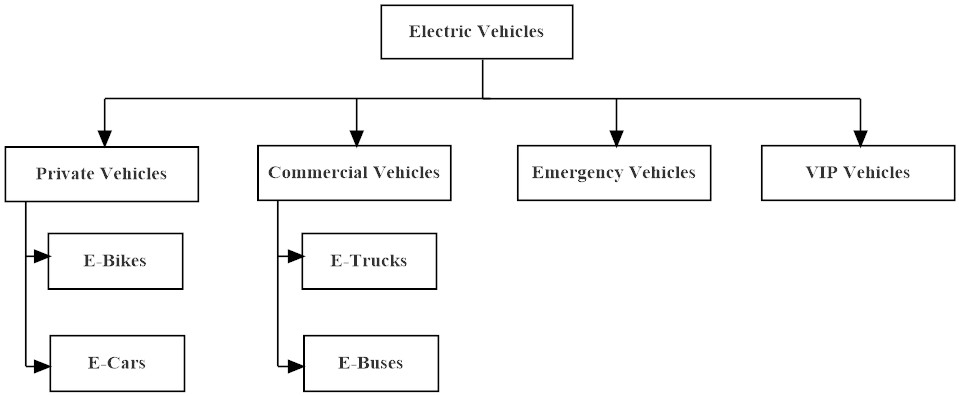
\includegraphics[width=0.7\linewidth]{./Figures/classification}
				\caption{Vehicle Classification}
				\label{fig:classification}
			\end{figure}
		
	The above classification is made by comparing the battery capacity of the vehicles from the data taken with the battery capacity of the similar kind of vehicles in the market.

	\par {Private vehicles are further classified into E-bikes and E-cars with average battery capacity of 400 $Wh$ to 500 $Wh$ and 40 $kWh$ to 100 $kWh$ respectively. Commercial vehicles are classified into E-Truck and E-Bus with an average battery capacity of 100 $kWh$ and 60 to 548 $kWh$ respectively. Emergency vehicles have a battery capacity of around 105 $kWh$ and VIP vehicles have around 90 $kWh$ to 200 $kWh$.
	}
	
	\section{Travel Pattern Establishment}
	
	Travel pattern for three main vehicle subcategories of the above mentioned vehicle categories namely E-car, E-Truck and E-Bus are now taken and travel patterns of the same have been established by using the Battery capacity, Time taken to full charge, Time period of the vehicle when it is connected to the grid , charging rate and discharging rate \cite{evdata}.
	
	Car: ID – 13646 \cite{evdata} is chosen for E-Car as its battery capacity matches with the most common types of E-cars in the market. The
	battery capacity range of this vehicle is 54 $kWh$. The time taken for 100\% charging of battery
	happens to be 1 hour 40 minutes. It then continues to Travel for 6 hour 30 minutes after which the Battery's Charge of the vehicle is depleted. This vehicle is connected to the grid for 5 hours 20 minutes until the next trip. The charging/discharging rate is 10.8 $kW$ per twenty minutes.
	
	Truck: ID – 4428 \cite{evdata} is chosen for E-Truck as its battery capacity matches with the most common types of E-Trucks in the market. The
	battery capacity of this vehicle is 99.2 $kWh$. The time taken for 100\% charging of battery
	happens to be 4 hours. It then continues to Travel for 14 hours after which the Battery's Charge of the vehicle is depleted. This vehicle is connected to the grid for 10 hours until the next trip. The charging/discharging rate is 8.267 $kW$ per twenty minutes.
	
	Bus: Vehicle ID – 16034 \cite{evdata} is chosen for E-bus as its battery capacity matches with the most common types of E-Buses in the market. The
	battery capacity of this vehicle is 199.95 $kWh$. The time taken for 100\% charging of battery
	happens to be 5 hours 20 minutes. It then continues to Travel for 13 hours after which the Battery's Charge of the vehicle is depleted. This vehicle is connected to the grid for 11 hours until the next trip. The charging/discharging rate is 12.5 $kW$ per twenty minutes.
	



	\section{Charging/Discharging Pattern Establishment}
	
	A 24 hour time scale is taken for charging/discharging pattern formulation. This time scale is further subdivided into 72 time blocks as the classified vehicles have non-uniform charging time, thereby rounding of time into hourly basis would be inefficient and unprecise. So inorder to increase precision, the 24 hour scale is split into 72 Blocks.
	
	\noindent Inorder to find the best charging/discharging/idle pattern equation \eqref{bestpattern} is used and this pattern provides less loss to the grid and is useful to the vehicle owner interms of cost.
	
	\noindent After running through all successive time logs of vehicles the whole data is analysed with this equation \eqref{argmin} and the connection time which is most profitable for both user and grid is identified.
	
	
	\section{Flowchart}
	
	\begin{enumerate}
		
		\item Data necessary for the EV charging is collected from the device and the time period for which it will be connected to the grid from the user.
		
		\item $SoC_{residual,t}$ is calculated from checking the vehicle's battery.
		
		\item This $SoC_{residual,t}$ is then compared with the $SoC_{threshold,t}$ to determine either to charge or discharge.
		
	
		\begin{enumerate}

			 \item 
			
			 \item
		
		\end{enumerate}
	\end{enumerate}
	
	\begin{figure}
		\centering
		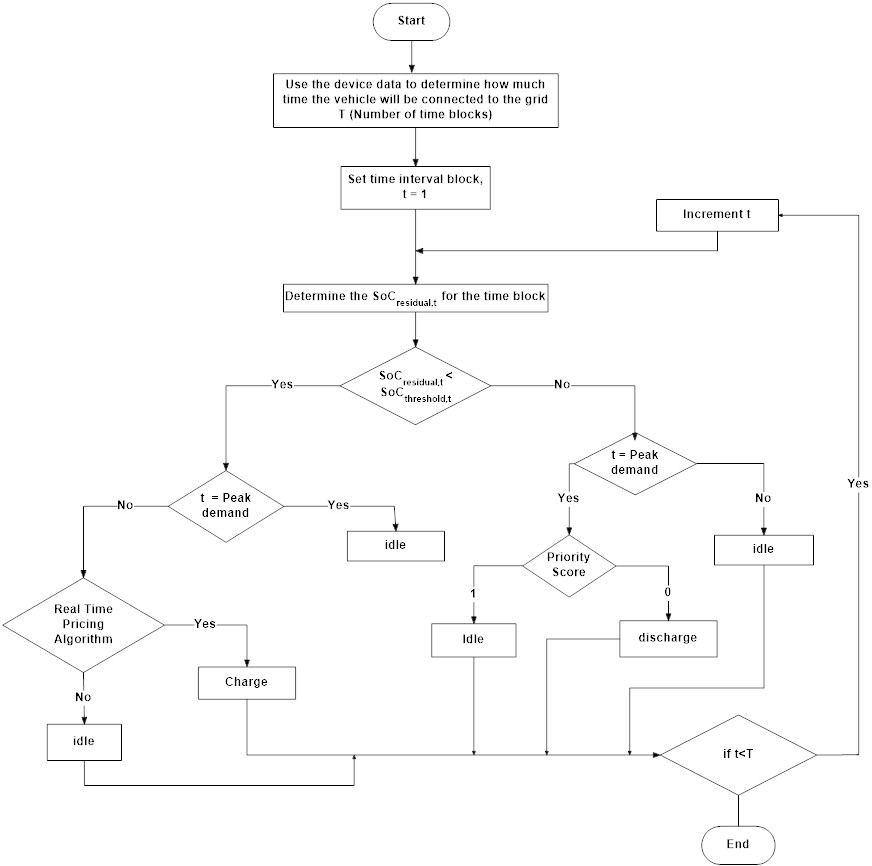
\includegraphics[width=0.9\linewidth]{Figures/Ev_flowchart}
		\caption{}
		\label{fig:evflowchart}
	\end{figure}


	\section{Real Time Price}
	
		\begin{figure}[!h]
			\centering
			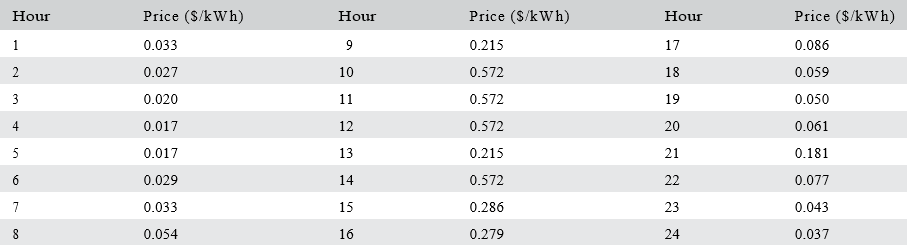
\includegraphics[width=0.7\linewidth]{Figures/rtp}
			\caption{}
			\label{fig:rtp}
		\end{figure}
	\section{Load Profile}
		\begin{figure}
			\centering
			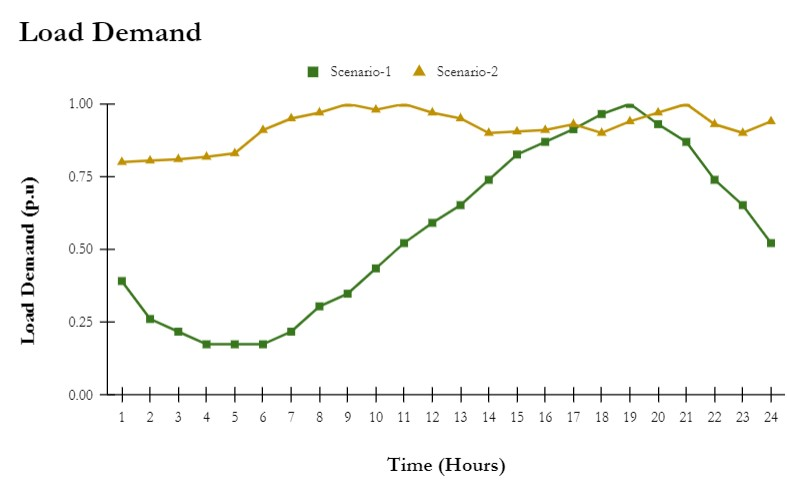
\includegraphics[width=0.7\linewidth]{C:/Users/HP/Downloads/load_demand}
			\caption{}
			\label{fig:loaddemand}
		\end{figure}
		
	
		
	
	
	
		\chapter{MATHEMATICAL MODELLING}
	\label{chap:mathmodel}
	This chapter deals with the Mathematical models involved in the SoC calculation, Charging pattern identification and maximum power demand created by the inclusion of EVs.
	
	\section{SoC Calculation}
	
	
		
	The SoC of the vehicle is calculated from the following equations:
	

			\begin{equation}
		                             SoC_{min} \leq SoC \leq SoC_{max}\label{eq:socminmax}
		    \end{equation}
	    
where `$SoC_{min}$'  and `$SoC_{max}$' are the minimum and maximum values of SoC and the values are 20 \% and 80 \% respectively.
		    \begin{equation}                         
		               SoC_{y} = SoC_{y-1} + P_{batt}(y) \times \partial y \times \eta c
			\end{equation}
		
		Where `$SoC_{y}$' is the state of charge in present hour and `$SoC_{y-1}$' is the state of charge in the previous hour. `$P_{battery}(y)$' represents the power of the battery in the present hour. `$\partial y$' is the time interval and `$\eta c$' is the charging efficiency which is considered to be 100 \%. 
		
		    \begin{equation}             
		               SoC_{y} = SoC_{y-1} - P_{batt}(y) \times \partial y \times \eta d
			\end{equation}
		
		Where `$SoC_{y}$' is the state of charge in present hour and `$SoC_{y-1}$' is the state of charge in the previous hour. `$P_{battery}(y)$' represents the power of the battery in the present hour. `$\partial y$' is the time interval and `$\eta d$' is the discharging efficiency which is considered to be 100 \%.
		
		    \begin{equation}             
		               P_{batt}(y) = SoC_{y} \times E
		    \end{equation}
	    
	    $P_{battery}(y)$' represents the output power of the battery in the present hour, `$SoC_{y}$' is the state of charge in present hour and $E$ is the energy of the battery. 
		 
\begin{equation}             
	 Initial Power = Generation - Load
\end{equation}

	  SoC limits:  
	 
	   $SoC_{min}$ and $SoC_{max}$ are  the maximum and minimum SoC of the EV respectively.
	   This constraint allows the SoC to vary between predefined minimum and maximum SoC.               
	
	\section{Best Pattern for charging}
	\label{chap:best}
	
	The charging pattern is determined by comparing the Energy required to the Real Time Price and by  identifying the minimum of it. 
	
	\begin{equation}
		\begin{split}
				T_{n} = \sum_{t=1}^{24} [Ch_{t} \times [1 || 0 || -1 ] ] \ast  Rtp_{t} 
		\end{split}
		\label{eqn:bestpattern}
    \end{equation}	 

where `$T_{n}$' is the cost of `$n^{th}$' iteration, `$i$' ranges from 1 to 24, `$Ch_{t}$' is the energy delivered at time `$t$' and `$Rtp_{t}$' is the real time price at the `$t^{th}$' time interval.

\noindent where `$[ \ 1 \ ||\ 0 \ ||\ -1\ ]$' represents the priority score for charging the vehicles.

	\begin{itemize}
		\item `1' - representing Charging
		\item `0' - representing idle
		\item `-1' - representing discharging
	\end{itemize}

\begin{equation}
	Charging \ Pattern = argmin (T_{n})
	\label{eqn:argmin}
\end{equation}	

The function `$argmin$'  is used to find the minimum cost from all the `$n$' iterations.	

	\section{Maximum Power required by EV}
	
	
	Maximum Power demand occurs when all the three vehicles loads are high and the time block of maximum demand is identified. 
	\begin{equation}
		\begin{split}
					P_{t(total)} = P_{t(car)} + P_{t(truck)} + P_{t(bus)}
		\end{split}
	\end{equation}	
where `$P_{t(car)}$', `$P_{t(truck)}$', `$P_{t(bus)}$' are the total power of car , truck and bus in $kW$ respectively. `$P_{t(total)}$' is the addition of the total  power of the individual vehicles (i.e.) car , truck and bus.
	\begin{equation}
		\begin{split}
				P_{t(total)} = argmax ~~\prod_{i=1}^{24} \ast P_{t(total)}
		\end{split}
	\end{equation}

`$P_{t(total)}$' is the addition of the total  power of the individual vehicles (i.e.) car , truck and bus. 
The function `$argmax$' is used to find the value of power from the total power. 
	

	
	
	\chapter{RESULTS \& DISCUSSION}
	\label{chap:results}
		In this chapter the inclusion of EVs and its impact of power loss in the presence of loads in the system is analyzed.
		

		
		
		
	\section{Simulation Outputs}
	The datas given below are about the Most Economic Time interval to Charge the Vehicle, charging Patterns and Voltage magnitude graphs for different scenarios.
			\subsection{Charging Patterns}
	These plots depict the charging and discharging pattern for the classified vehicles. 216 vehicles are taken into consideration for each vehicle type and the charging pattern is identified.
	
	
	
	\begin{figure}[!h]
		\centering
		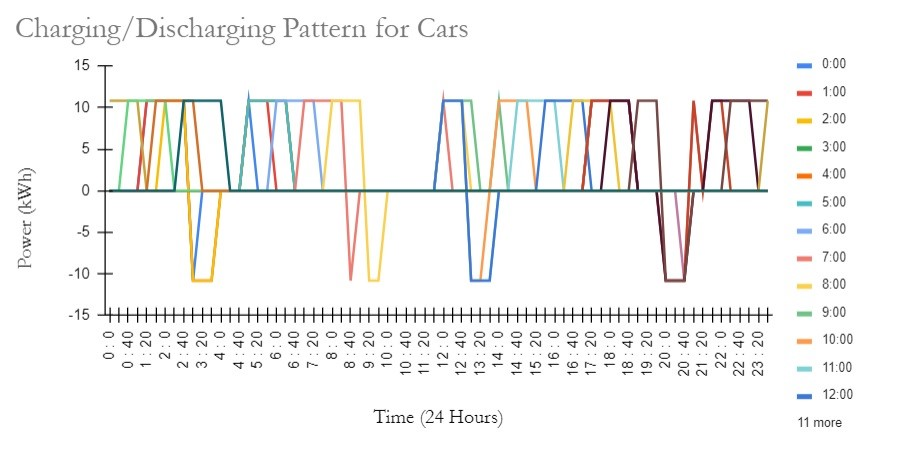
\includegraphics[width=0.7\linewidth]{Figures/cp_case1}
		\caption{Charging/Discharging pattern for Cars}
		\label{fig:cpcase1}
	\end{figure}
	
	\begin{figure}[!h]
		\centering
		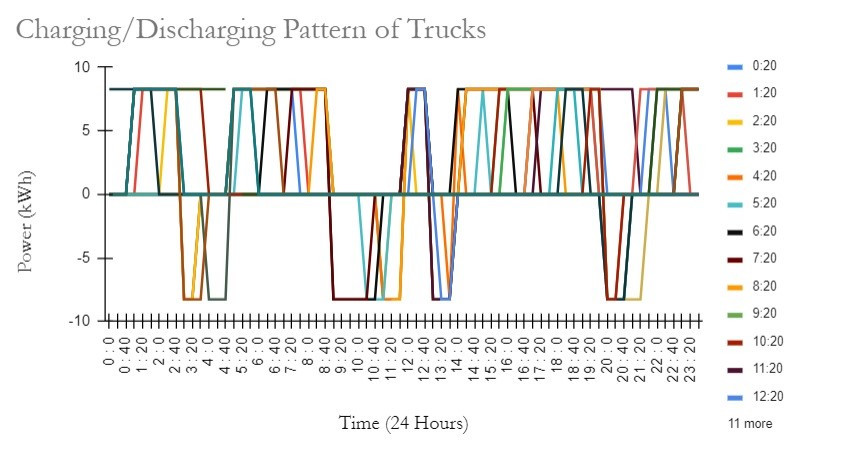
\includegraphics[width=0.7\linewidth]{Figures/cp_case2}
		\caption{Charging/Discharging pattern for Trucks}
		\label{fig:cpcase2}
	\end{figure}
	
	\begin{figure}[!h]
		\centering
		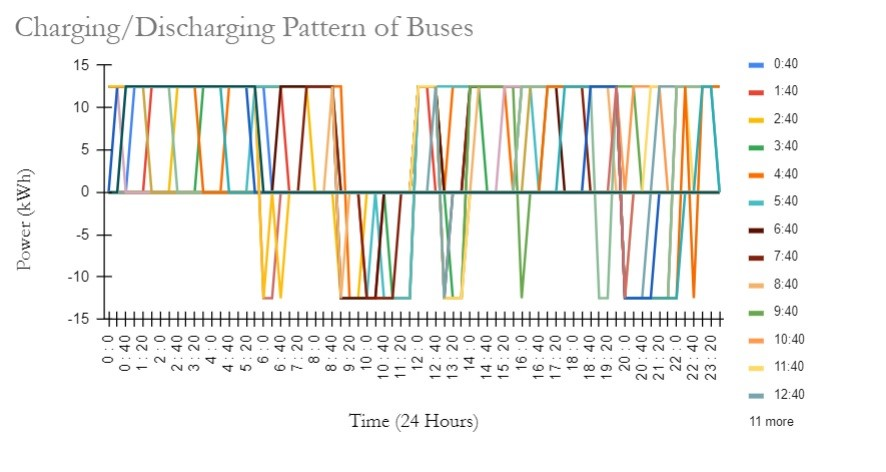
\includegraphics[width=0.7\linewidth]{Figures/cp_case3}
		\caption{Charging/Discharging pattern for Buses}
		\label{fig:cpcase3}
	\end{figure}
	
	\noindent A strategic pattern is established to maintain the stability of the grid by comparing the vehicle capacity to the Real time price for each hour. When the price is low, the vehicle is put to charge and when the price is high,the vehicle is put to discharge in comparision with the peak demand. By this way the overall cost is drastically reduced , leading to profit for the user and at the same time the overall load in the grid decreases making the load demand curve flatter.
	
	
		\subsection{Economic Charging}
		
			Three cases are taken in this study which are namely:
				\newline Case 1(00:00): Case 1 depicts that the vehicles has Started on a hourly basis i.e. the 1 hour block.
				\newline Case 2(00:20) : Case 2 depicts that the vehicle has Started from the 20th min of an hour i.e. 20mins block.
				\newline Case 3(00:40): Case 3 depicts that the vehicles has Started from the 40th minute of an hour i.e. 40th minute block
			
			\begin{table}[!h]
				\caption{Most Economic Time interval to Charge the Vehicle}
				\centering
			\begin{tabular}{|l|l|l|l|}
				\hline
				\textbf{VEHICLE TYPE}           & \textbf{CASE}         & \textbf{BEST PRICE} & \textbf{HOUR} \\ \hline
				\multirow{3}{*}{\textbf{CAR}}   & \textbf{Case 1 - (00:00)} & - \$1.71            & 12:00         \\ \cline{2-4} 
				& \textbf{Case 2 - (00:20)} & - \$2.09            & 01:20         \\ \cline{2-4} 
				& \textbf{Case 3 - (00:40)} & - \$1.58            & 01:40         \\ \hline
				\multirow{3}{*}{\textbf{BUS}}   & \textbf{Case 1 - (00:00)} & - \$0.47            & 12:00         \\ \cline{2-4} 
				& \textbf{Case 2 - (00:20)} & - \$1.25            & 20:20         \\ \cline{2-4} 
				& \textbf{Case 3 - (00:40)} & - \$0.69            & 11:40         \\ \hline
				\multirow{3}{*}{\textbf{TRUCK}} & \textbf{Case 1 - (00:00)} & - \$2.57            & 05:00         \\ \cline{2-4} 
				& \textbf{Case 2 - (00:20)} & -\$1.00             & 04:20         \\ \cline{2-4} 
				& \textbf{Case 3 - (00:40)} & - \$2.11            & 04:40         \\ \hline
			\end{tabular}
		\label{table:ec}
		\end{table}
		
		

	%\subsection{Maximum EV Load}
	
		In the table \ref{table:whichbus} the hour at which the maximum load is present is shown for Scenario-1 and Scenario-2 along with the load present in the system.
		
			\begin{table}[!h]
			\centering
			\caption{Hour at which the EV Load is maximum }
			\begin{tabular}{|ll|ll|ll|ll|}
				\hline
				\multicolumn{2}{|l|}{\textbf{Scenario}} & \multicolumn{2}{l|}{\textbf{Case-1}} & \multicolumn{2}{l|}{\textbf{Case-2}} & \multicolumn{2}{l|}{\textbf{Case-3}} \\ \hline
				\multicolumn{2}{|l|}{\textbf{Scenario-1}}        & \multicolumn{2}{l|}{$ 19^{th} $}            & \multicolumn{2}{l|}{$ 6^{th} $}             & \multicolumn{2}{l|}{$ 19^{th} $}             \\ \hline
				\multicolumn{2}{|l|}{\textbf{Scenario-2}}        & \multicolumn{2}{l|}{$ 13^{th} $}           & \multicolumn{2}{l|}{$ 6^{th} $}             & \multicolumn{2}{l|}{$ 13^{th} $}             \\ \hline
			\end{tabular}
			\label{table:whichbus}
		\end{table}
	

	
	\section{33 bus system}
		In the 33 bus system the EVs are placed at buses 2 (Strongest Bus) and 18 (Weakest Bus) with Voltage Stability Index as a consideration \cite{33bus} .
 		In the provided table \ref{table:powerloss} the power losses are calculated for the corresponding time blocks  as shown in table \ref{table:whichbus} along with the available loads for that particular hour. The results are tabulated in \ref{table:powerloss}.
 		The voltage magnitude of the base case and each time block for  all the cases are computed. Load flow analysis is done on Bus number 2 and Bus number 18 as these are considered to be the best case and worst case buses to calculate the voltage magnitude as referred from \cite{33bus}. From the results it is evident that the loss difference in the grid without EVs connected to the grid(base case) and with EVs connected to the grid on bus number 2 are comparatively lesser. The same loss difference is higher when the EVs connected in 18th bus is high. Looking into voltage magnitude the value of voltage magnitude in base case and EVs connected to the grid on 2nd bus are equal. Whereas in 18th bus it is clear that voltage magnitude when compared to base case is high.
 		
 		\noindent Here figures (\ref{fig:LFa}), (\ref{fig:LFb}) and  (\ref{fig:LFc}) shows the voltage magnitude plot when the EVs are connected to bus 2 and bus 18 during various cases.
 		
 		\noindent and figures (\ref{fig:LF2a}), (\ref{fig:LF2b}) and  (\ref{fig:LF2c}) shows the voltage magnitude plot when the EVs are connected to bus 2 and bus 18 during various cases.
 		
 		
 		
 		
 		
 		\noindent The base case power loss of the 33 bus system is 202.691 `$kWh$' i.e. when the load demand is 100 percent. The summation of all 72 individual loads of cars, trucks and buses for each case is calculated. These additive loads are identified in each time block and the maximum of it is taken into calculation for load flow.

 		\textbf{Case 1:}
 			\begin{itemize}
 				\item Case one is the hourly connection of vehicles starting at 00:00 and the peak load of EVs is found at $19^{th}$ hour with a load of 284.97 $kW$ 
 				\item This load is connected in bus 2 and bus 18 under two different scenarios with active load demand 1 and 0.94 respectively.
 				\item The resulting power loss is 204.104 $kW$ and 253.746 $kW$ respectively for scenario 1 and 189.833 $kW$ and 236.912 $kW$ respectively for scenario 2.
 				\item This shows a 24.49 percent higher loss in scenario 1 and 10.54 percent higher loss in scenario 2.
 			\end{itemize}

 		\textbf{Case 2:}
 		\begin{itemize}
 			\item Case two is the hourly  connection of vehicles starting at 00:20 and the peak load of EVs is found at $6^{th}$ hour with a load of 276.703 $kW$ 
 			\item This load is connected in bus 2 and bus 18 under two different scenarios with active load demand 0.173913043 and 0.83 respectively.
 			\item The resulting power loss is 65.773 $kW$ and 78.460 $kW$ respectively for scenario 1 and 178.967 $kW$ and 222.468 $kW$ respectively for scenario 2.
 			\item This shows a 6.26 percent higher loss in scenario 1 and 1.943 percent higher loss in scenario 2.
 		\end{itemize}
 		
 		\textbf{Case 3:}
 		\begin{itemize}
 			\item Case three is the hourly connection of vehicles starting at 00:40 and the peak load of EVs is found at $19^{th}$ hour with a load of 284.97 $kW$ 
 			\item This load is connected in bus 2 and bus 18 under two different scenarios with active load demand 1 and 0.94 respectively.
 			\item The resulting power loss is 204.104 $kW$ and 253.746 $kW$ respectively for scenario 1 and 189.833 $kW$ and 236.912 $kW$ respectively for scenario 2.
 			\item This shows a 24.49 percent higher loss in scenario 1 and 10.54 percent higher loss in scenario 2.
 		\end{itemize}
 		
 		From the figure \ref{fig:loadprofile33},  we can identify that the difference in voltage magnitudes differ highly from the base case on the $18^{th}$ bus and remains almost constant on the $2^{nd}$ bus, this concludes that Bus 18 is the weakest bus and Bus 2 isthe strongest bus in this 33 bus system. 
 		
 		
 		
 		
 		
 		
 		
 		
 		
 		
 		
 		
 		
 		
 		
 				\begin{table}[!t]
 			\centering
 			\caption{Power Loss when EV is connected in a 33 bus system}
 			\begin{tabular}{|c|c|cc|cc|cc|}
 				\hline
 				\multirow{2}{*}{\textbf{Scenario}}                            & \multirow{2}{*}{\textbf{\begin{tabular}[c]{@{}c@{}}Base\\ Case\\ Power\\ Loss\\ (kW)\end{tabular}}} & \multicolumn{2}{c|}{\textbf{Case 1}}                                                                                                                                                                          & \multicolumn{2}{c|}{\textbf{Case 2}}                                                                                                                                                                          & \multicolumn{2}{c|}{\textbf{Case 3}}                                                                                                                                                                          \\ \cline{3-8} 
 				&                                                                                              & \multicolumn{1}{c|}{\textbf{\begin{tabular}[c]{@{}c@{}}Power \\ Loss\\ when EV\\ in Bus 2\\ (kW)\end{tabular}}} & \textbf{\begin{tabular}[c]{@{}c@{}}Power \\ Loss\\ when EV\\ in Bus 18\\ (kW)\end{tabular}} & \multicolumn{1}{c|}{\textbf{\begin{tabular}[c]{@{}c@{}}Power \\ Loss\\ when EV\\ in Bus 2\\ (kW)\end{tabular}}} & \textbf{\begin{tabular}[c]{@{}c@{}}Power \\ Loss\\ when EV\\ in Bus 18\\ (kW)\end{tabular}} & \multicolumn{1}{c|}{\textbf{\begin{tabular}[c]{@{}c@{}}Power\\  Loss\\ when EV\\ in Bus 2\\ (kW)\end{tabular}}} & \textbf{\begin{tabular}[c]{@{}c@{}}Power \\ Loss\\ when EV\\ in Bus 18\\ (kW)\end{tabular}} \\ \hline
 				\textbf{\begin{tabular}[c]{@{}c@{}}Scenario\\ 1\end{tabular}} & \multirow{2}{*}{202.691}                                                                     & \multicolumn{1}{c|}{204.104}                                                                                    & 253.746                                                                                     & \multicolumn{1}{c|}{65.773}                                                                                     & 78.460                                                                                      & \multicolumn{1}{c|}{204.104}                                                                                    & 253.746                                                                                     \\ \cline{1-1} \cline{3-8} 
 				\textbf{\begin{tabular}[c]{@{}c@{}}Scenario\\ 2\end{tabular}} &                                                                                              & \multicolumn{1}{c|}{189.833}                                                                                    & 236.912                                                                                     & \multicolumn{1}{c|}{178.967}                                                                                    & 222.468                                                                                     & \multicolumn{1}{c|}{189.833}                                                                                    & 236.912                                                                                     \\ \hline
 			\end{tabular}
 			\label{table:powerloss}
 		\end{table}
 	
 		\begin{figure}[!h]
 			\begin{subfigure}{.5\textwidth}
 				\centering
 				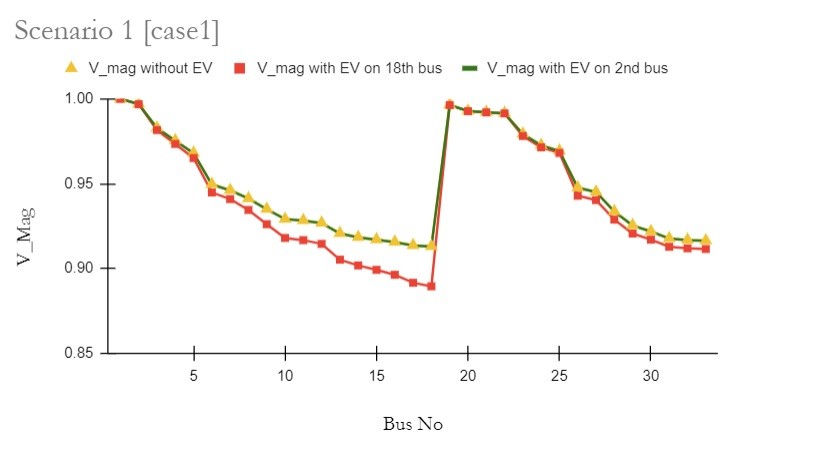
\includegraphics[width=.97\linewidth,height= 4.95cm]{./Figures/sc1_case1}  
 				\caption{Case I}
 				\label{fig:LFa}
 			\end{subfigure}
 			\begin{subfigure}{.5\textwidth}
 				\centering
 				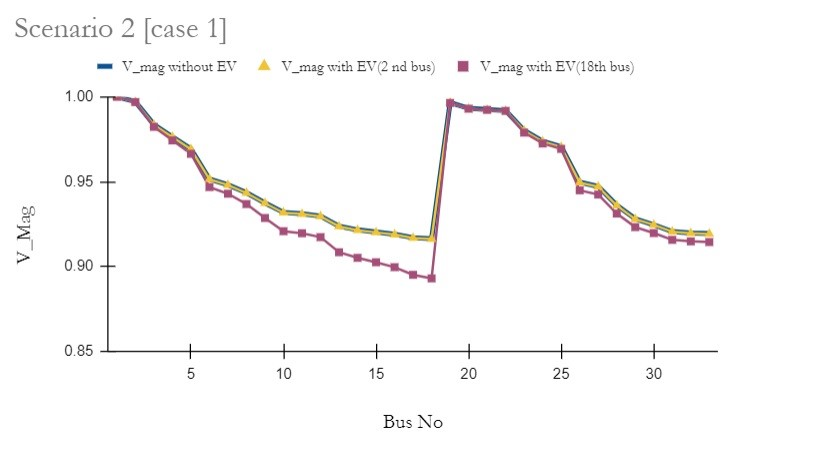
\includegraphics[width=.97\linewidth,height= 4.95cm]{./Figures/sc2_case1}  
 				\caption{Case I}
 				\label{fig:LF2a}
 			\end{subfigure}
 			\begin{subfigure}{.5\textwidth}
 				\centering
 				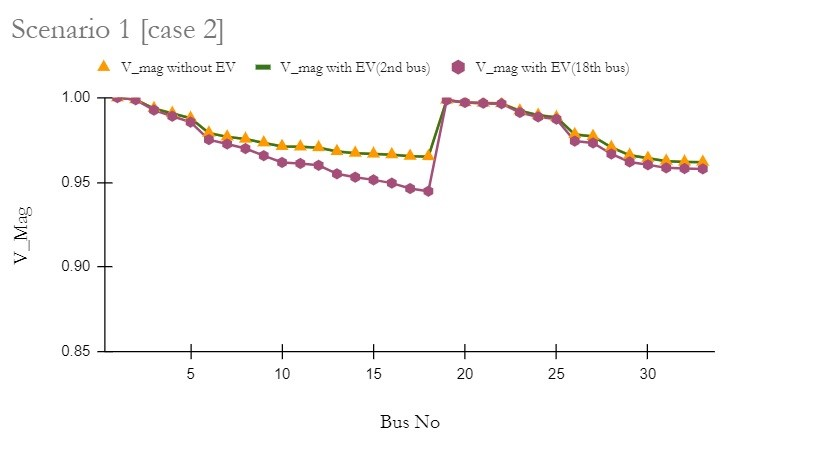
\includegraphics[width=.97\linewidth,height= 4.95cm]{./Figures/sc1_case2}
 				\caption{Case II}
 				\label{fig:LFb}
 			\end{subfigure}
 			\begin{subfigure}{.5\textwidth}
 				\centering
 				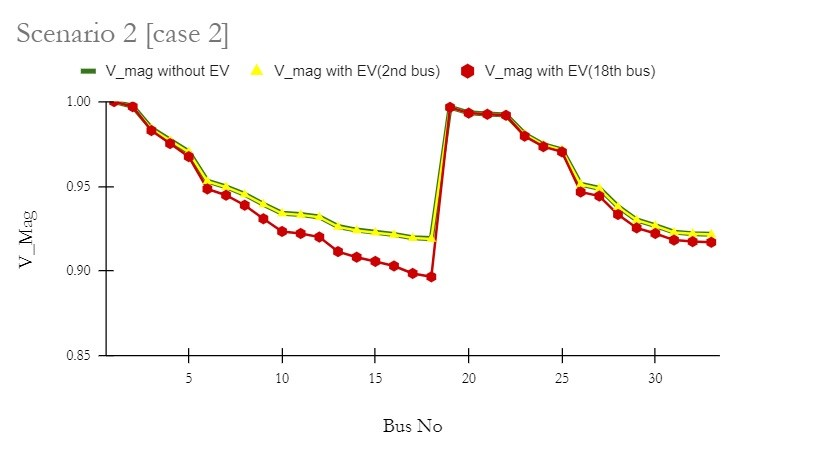
\includegraphics[width=.97\linewidth,height= 4.95cm]{./Figures/sc2_case2}
 				\caption{Case II}
 				\label{fig:LF2b}
 			\end{subfigure}
 			\begin{subfigure}{.5\textwidth}
 				\centering
 				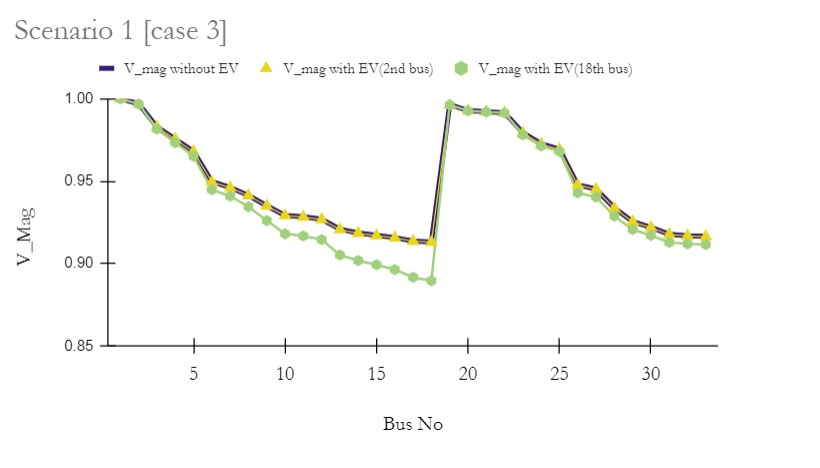
\includegraphics[width=.97\linewidth,height= 4.95cm]{./Figures/sc1_case3}
 				\caption{Case III}
 				\label{fig:LFc}
 			\end{subfigure}
 			\begin{subfigure}{.5\textwidth}
 				\centering
 				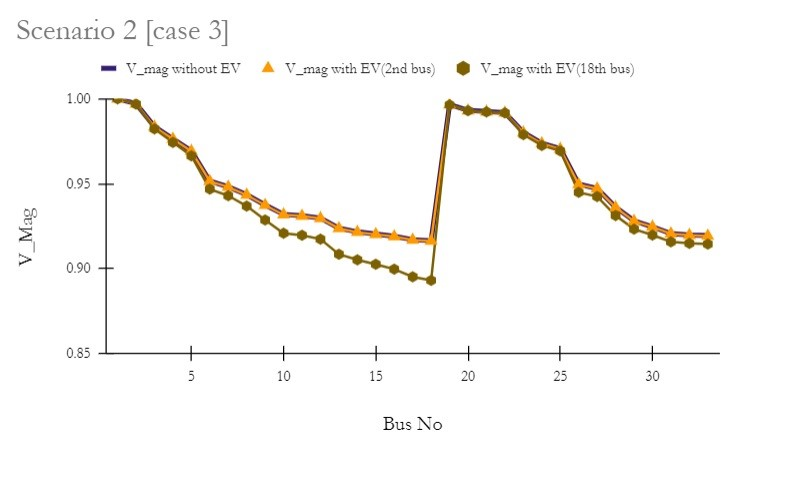
\includegraphics[width=.97\linewidth,height= 4.95cm]{./Figures/sc2_case3}
 				\caption{Case III}
 				\label{fig:LF2c}
 			\end{subfigure}
 			\caption{ Voltage magnitude variation for different scenarios on 33 bus system }
 			\label{fig:loadprofile33}
 		\end{figure} 
 		
		
	



	\section{69 bus system}
In the provided table \ref{table:powerloss69} the power loss is calculated in such a way that the time blocks having the maximum load  is considered and then load flow analysis is performed on 2nd bus(best case)and 54th bus (worst case) of 69 bus system to find the variation of load with and without EV .


\begin{table}[!h]
				\centering
	\caption{Power Loss when EV is connected in a 69 bus system}
	\begin{tabular}{|c|c|cc|cc|cc|}
		\hline
		\multirow{2}{*}{\textbf{Scenario}}                            & \multirow{2}{*}{\textbf{\begin{tabular}[c]{@{}c@{}}Base\\ Case\\ Power\\ Loss\\ (kW)\end{tabular}}} & \multicolumn{2}{c|}{\textbf{Case 1}}                                                                                                                                                                          & \multicolumn{2}{c|}{\textbf{Case 2}}                                                                                                                                                                          & \multicolumn{2}{c|}{\textbf{Case 3}}                                                                                                                                                                          \\ \cline{3-8} 
		&                                                                                              & \multicolumn{1}{c|}{\textbf{\begin{tabular}[c]{@{}c@{}}Power \\ Loss\\ when EV\\ in Bus 2\\ (kW)\end{tabular}}} & \textbf{\begin{tabular}[c]{@{}c@{}}Power \\ Loss\\ when EV\\ in Bus 54\\ (kW)\end{tabular}} & \multicolumn{1}{c|}{\textbf{\begin{tabular}[c]{@{}c@{}}Power \\ Loss\\ when EV\\ in Bus 2\\ (kW)\end{tabular}}} & \textbf{\begin{tabular}[c]{@{}c@{}}Power \\ Loss\\ when EV\\ in Bus 54\\ (kW)\end{tabular}} & \multicolumn{1}{c|}{\textbf{\begin{tabular}[c]{@{}c@{}}Power\\  Loss\\ when EV\\ in Bus 2\\ (kW)\end{tabular}}} & \textbf{\begin{tabular}[c]{@{}c@{}}Power \\ Loss\\ when EV\\ in Bus 54\\ (kW)\end{tabular}} \\ \hline
		\textbf{\begin{tabular}[c]{@{}c@{}}Scenario\\ 1\end{tabular}} & \multirow{2}{*}{226.28}                                                                      & \multicolumn{1}{c|}{207.402}                                                                                    & 220.681                                                                                     & \multicolumn{1}{c|}{198.458}                                                                                      & 210.909                                                                                     & \multicolumn{1}{c|}{207.402}                                                                                    & 220.681                                                                                     \\ \cline{1-1} \cline{3-8} 
		\textbf{\begin{tabular}[c]{@{}c@{}}Scenario\\ 2\end{tabular}} &                                                                                              & \multicolumn{1}{c|}{134.758}                                                                                    & 144.014                                                                                     & \multicolumn{1}{c|}{77.01}                                                                                    & 77.1223                                                                                     & \multicolumn{1}{c|}{134.758}                                                                                    & 144.014                                                                                     \\ \hline
	\end{tabular}
	\label{table:powerloss69}
\end{table}


The voltage magnitude of the base case and each time block for  all the cases are computed. Load flow analysis is done on Bus number 2 and Bus number 54 as these are considered to be the best case and worst case buses to calculate the voltage magnitude as referred from \cite{base}. From the results it is evident that the loss difference in the grid without EVs connected to the grid(base case) and with EVs connected to the grid on bus number 2 are comparatively lesser. The same loss difference is higher when the EVs connected in 54th bus is high. Looking into voltage magnitude the value of voltage magnitude in base case and EVs connected to the grid on 2nd bus are equal. Whereas in 18th bus it is clear that voltage magnitude when compared to base case is high.

\noindent Here figures (\ref{fig:RFa}), (\ref{fig:RFb}) and  (\ref{fig:RFc}) shows the voltage magnitude plot when the EVs are connected to bus 2 and bus 18 during various cases.

\noindent and figures (\ref{fig:RF2a}), (\ref{fig:RF2b}) and  (\ref{fig:RF2c}) shows the voltage magnitude plot when the EVs are connected to bus 2 and bus 18 during various cases.

\begin{figure}[!h]
	\begin{subfigure}{.5\textwidth}
		\centering
		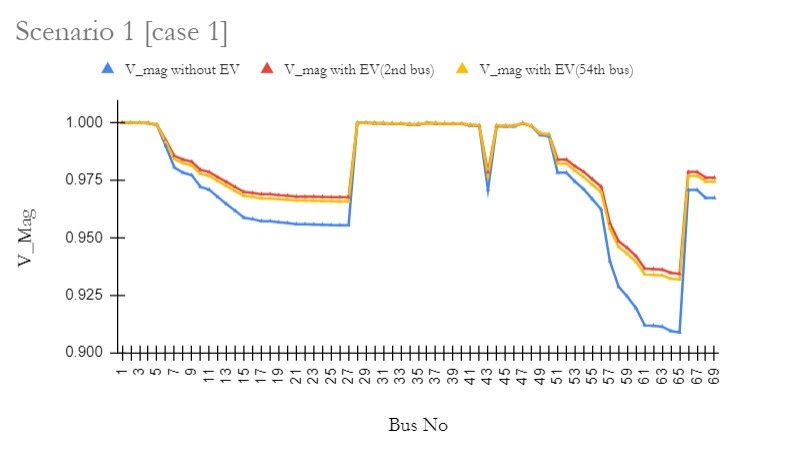
\includegraphics[width=.97\linewidth,height= 4.95cm]{./Figures/69_sc1_case1}  
		\caption{Case I}
		\label{fig:RFa}
	\end{subfigure}
	\begin{subfigure}{.5\textwidth}
		\centering
		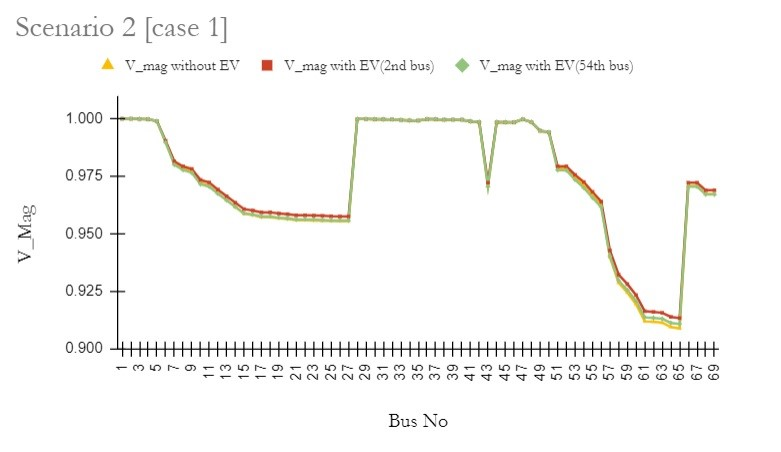
\includegraphics[width=.97\linewidth,height= 4.95cm]{./Figures/69_sc2_case1}  
		\caption{Case I}
		\label{fig:RF2a}
	\end{subfigure}
	\begin{subfigure}{.5\textwidth}
		\centering
		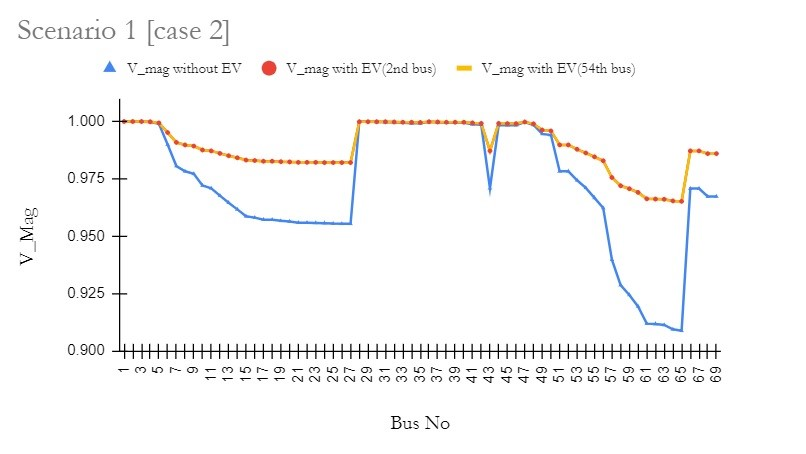
\includegraphics[width=.97\linewidth,height= 4.95cm]{./Figures/69_sc1_case2}
		\caption{Case II}
		\label{fig:RFb}
	\end{subfigure}
	\begin{subfigure}{.5\textwidth}
		\centering
		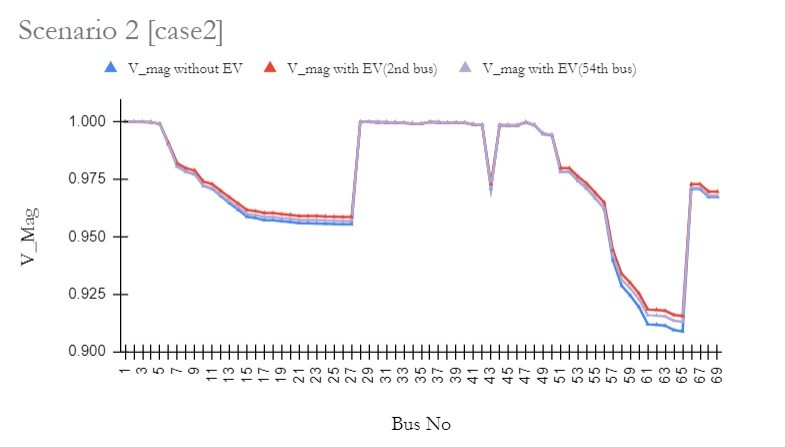
\includegraphics[width=.97\linewidth,height= 4.95cm]{./Figures/69_sc2_case2}
		\caption{Case II}
		\label{fig:RF2b}
	\end{subfigure}
	\begin{subfigure}{.5\textwidth}
		\centering
		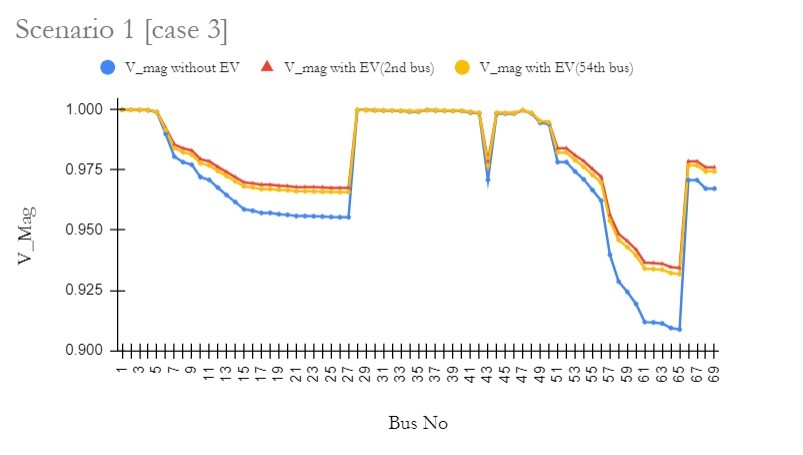
\includegraphics[width=.97\linewidth,height= 4.95cm]{./Figures/69_sc1_case3}
		\caption{Case III}
		\label{fig:RFc}
	\end{subfigure}
	\begin{subfigure}{.5\textwidth}
		\centering
		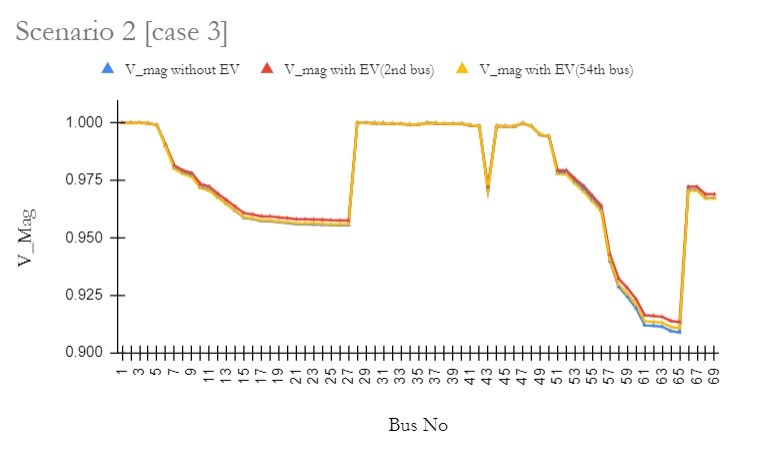
\includegraphics[width=.97\linewidth,height= 4.95cm]{./Figures/69_sc2_case3}
		\caption{Case III}
		\label{fig:RF2c}
	\end{subfigure}
	\caption{ Voltage magnitude variation for different scenarios on 69 bus system  }
	\label{fig:loadprofile69}
\end{figure} 
	
	


		
	
	
	
	
		\chapter{CONCLUSIONS AND FURTHER WORK}
	\label{chap:conclusion}
	
	
	Therefore in this study we have classeified the Electric Vehicles, determined their Travel Pattern, estimated their Charging/Discharging Pattern with the help of `$Rtp$', thereby finding the best time period to charge the vehicle with respect to cost for the considered data and have verified that, when the the EVs are connected to a strong bus the losses are less and viceversa.
	
	
	\vspace*{24pt}
	
	\noindent \textbf{Signature of the Guide} \hspace*{69mm} \textbf{Student Reg. No:}123005085\\
		\\
	\\
	\\
\noindent \textbf{Name of the Guide}:{ Dr.~Narayanan K}~(SAP/EEE/SEEE) \hspace*{7mm} \textbf{Name:}Mithra Vinda Reddy K
\pagebreak
	\pagebreak
	
	%%%%%%%%%%%%%%%%%%%%%%%%%%%%%%%%%%%%%%%%%%%%%%%%%%%%%%%%%%%%%%%%%
	% for the second member

	\begin{center}
		\Large{{\textbf{CONCLUSIONS}}}
	\end{center}
	Therefore in this study we have classeified the Electric Vehicles, determined their Travel Pattern, estimated their Charging/Discharging Pattern with the help of `$Rtp$', thereby finding the best time period to charge the vehicle with respect to cost for the considered data and have verified that, when the the EVs are connected to a strong bus the losses are less and viceversa.
	
	
	\vspace*{24pt}
	
	\noindent \textbf{Signature of the Guide} \hspace*{66mm} \textbf{Student Reg. No:}123005132\\
		\\
	\\
	\\
\noindent \textbf{Name of the Guide}:{ Dr.~Narayanan K}~(SAP/EEE/SEEE) \hspace*{10 mm} \textbf{Name:}Sarvesh Babu R G
\pagebreak
	\pagebreak
	
	
	%%%%%%%%%%%%%%%%%%%%%%%%%%%%%%%%%%%%%%%%%%%%%%%%%%%%%%%%%%%%
	% for the third member
	\begin{center}
		\Large{{\textbf{CONCLUSIONS}}}
	\end{center}
	
		\noindent Therefore in this study we have classeified the Electric Vehicles, determined their Travel Pattern, estimated their Charging/Discharging Pattern with the help of `$Rtp$', thereby finding the best time period to charge the vehicle with respect to cost for the considered data and have verified that, when the the EVs are connected to a strong bus the losses are less and viceversa.
	
	\vspace*{24pt}
	
		\noindent \textbf{Signature of the Guide} \hspace*{71mm} \textbf{Student Reg. No:}123005140\\
			\\
		\\
		\\
	\noindent \textbf{Name of the Guide}:{ Dr.~Narayanan K}~(SAP/EEE/SEEE) \hspace*{15mm} \textbf{Name:}Shwetha S
	\pagebreak
	\pagebreak
	
	
	%%%%%%%%%%%%%%%%%%%%%%%%%%%%%%%%%%%%%%%%%%%%%%%%%%%%%%%%%%%%
	%%%%%%%%%%%%%%%%%%%%%%%%%%%%%%%%%%%%%%%%%%%%%%%%%%%%%%%%%%%%%%%%%

% Bibliography.
\addcontentsline{toc}{chapter}{REFERENCES}
%\bibliographystyle{plain}
%\bibliography{mybib}
\begin{singlespace}
\bibliography{refs}
\end{singlespace}

% Appendices.
%%%%%%%%%%%%%%%%%%%%%%%%%%%%%%%%%%%%%%%%%%%%%%%%%%%%%%%%%%%%
\appendix
	\chapter{IEEE 33 BUS SYSTEM}
%\flushleft
This test system and its data are referred from \cite{rao}. In base case (i.e) topology I, there are five open tie switches and branch numbers are 33, 34, 35, 36, and 37 respectively. In topology II, the five open tie switches and branch numbers are 7, 9, 14, 32, and 37 respectively.  The single line diagram of the IEEE 33 bus system is shown in Fig. \ref{fig:single33}. The total real and reactive power loads on the system are 3715 $kW$ and 2300 $kVAr$ respectively. The voltage magnitude of the system is 1\angle\ang{0} p.u.

\begin{figure}[ht]
		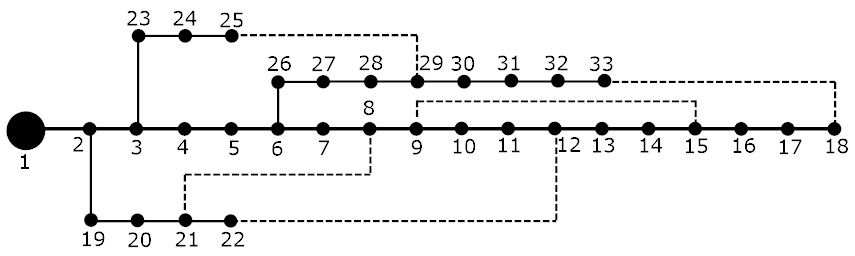
\includegraphics[width=1\textwidth]{./Figures/33bus_singleline_diagram_tieline_t1}
	\caption{Single line diagram of IEEE-33 Bus System}
	\label{fig:single33}
\end{figure}

\pagebreak
	\begin{longtable}{cccccccccc}
		\caption {IEEE 33 Bus System Bus Data}
		\label{table:busdata33}
		\hline
		\multirow{1}{*}{\begin{tabular}[c]{@{}c@{}}Bus \\ No.\end{tabular}} & \multirow{1}{*}{\begin{tabular}[c]{@{}c@{}}Bus \\ Code\end{tabular}} & \multirow{1}{*}{\begin{tabular}[c]{@{}c@{}}Load\\ Type\end{tabular}} & \multicolumn{2}{c}{Load} & \multicolumn{4}{c}{Generator} & \multirow{1}{*}{\begin{tabular}[c]{@{}c@{}}Injected \\ MVAr\end{tabular}} \\
		\cmidrule{4-5} 
		\cmidrule(lr{1em}){6-9}
		&  &  & \multirow{1}{*}{MW} & \multirow{1}{*}{MVAr} & \multirow{1}{*}{MW} & \multirow{1}{*}{MVAr} & \multirow{1}{*}{Qmin} & \multirow{1}{*}{Qmax} &  \\
		&  &  &  &  &  &  &  &  &  \\
		\cmidrule(lr){1-10}
		1 & 1 & -           & 0     & 0     & 0 & 0 & 0 & 0 & 0 \\
		2 & 0 & Curtailable & 0.100 & 0.060 & 0 & 0 & 0 & 0 & 0 \\
		3 & 0 & Curtailable & 0.090 & 0.040 & 0 & 0 & 0 & 0 & 0 \\
		4 & 0 & Curtailable & 0.120 & 0.080 & 0 & 0 & 0 & 0 & 0 \\
		5 & 0 & Curtailable & 0.060 & 0.030 & 0 & 0 & 0 & 0 & 0 \\
		6 & 0 & Fixed & 0.060 & 0.020 & 0 & 0 & 0 & 0 & 0 \\
		7 & 0 & Fixed & 0.200 & 0.100 & 0 & 0 & 0 & 0 & 0 \\
		8 & 0 & Fixed & 0.200 & 0.100 & 0 & 0 & 0 & 0 & 0 \\
		9 & 0 & Fixed & 0.060 & 0.020 & 0 & 0 & 0 & 0 & 0 \\
		10 & 0 & Fixed & 0.060 & 0.020 & 0 & 0 & 0 & 0 & 0 \\
		11 & 0 & Fixed & 0.045 & 0.020 & 0 & 0 & 0 & 0 & 0 \\
		12 & 0 & Controllable & 0.060 & 0.035 & 0 & 0 & 0 & 0 & 0 \\
		13 & 0 & Controllable & 0.060 & 0.035 & 0 & 0 & 0 & 0 & 0 \\
		14 & 0 & Controllable & 0.120 & 0.080 & 0 & 0 & 0 & 0 & 0 \\
		15 & 0 & Controllable & 0.060 & 0.010 & 0 & 0 & 0 & 0 & 0 \\
		16 & 0 & Controllable & 0.060 & 0.020 & 0 & 0 & 0 & 0 & 0 \\
		17 & 0 & Controllable & 0.060 & 0.020 & 0 & 0 & 0 & 0 & 0 \\
		18 & 0 & Controllable & 0.090 & 0.040 & 0 & 0 & 0 & 0 & 0 \\
		19 & 0 & Controllable & 0.090 & 0.040 & 0 & 0 & 0 & 0 & 0 \\
		20 & 0 & Controllable & 0.090 & 0.040 & 0 & 0 & 0 & 0 & 0 \\
		21 & 0 & Controllable & 0.090 & 0.040 & 0 & 0 & 0 & 0 & 0 \\
		22 & 0 & Controllable & 0.090 & 0.040 & 0 & 0 & 0 & 0 & 0 \\
		23 & 0 & Controllable & 0.090 & 0.050 & 0 & 0 & 0 & 0 & 0 \\
		24 & 0 & Controllable & 0.420 & 0.200 & 0 & 0 & 0 & 0 & 0 \\
		25 & 0 & Controllable & 0.420 & 0.200 & 0 & 0 & 0 & 0 & 0 \\
		26 & 0 & Curtailable & 0.060 & 0.025 & 0 & 0 & 0 & 0 & 0 \\
		27 & 0 & Curtailable & 0.060 & 0.025 & 0 & 0 & 0 & 0 & 0 \\
		28 & 0 & Curtailable & 0.060 & 0.020 & 0 & 0 & 0 & 0 & 0 \\
		29 & 0 & Curtailable & 0.120 & 0.070 & 0 & 0 & 0 & 0 & 0 \\
		30 & 0 & Curtailable & 0.200 & 0.600 & 0 & 0 & 0 & 0 & 0 \\
		31 & 0 & Curtailable & 0.150 & 0.070 & 0 & 0 & 0 & 0 & 0 \\
		32 & 0 & Curtailable & 0.210 & 0.100 & 0 & 0 & 0 & 0 & 0 \\
		33 & 0 & Curtailable & 0.060 & 0.040 & 0 & 0 & 0 & 0 & 0 \\
	\bottomrule %[1.5pt]		
\end{longtable}
\begin{flushleft}
	%\flushleft
	\item  Bus Code
	\newline 1 - Slack Bus \newline 0 - Load Bus
	
\end{flushleft}	

	\begin{longtable}{ccccccccc}
	\caption {IEEE 33 Bus System Line Data}
	\label{table:linedata33}
	\hline
	\multirow{4}{*}{\begin{tabular}[c]{@{}c@{}}  Line \\ No.\end{tabular}} & \multirow{4}{*}{\begin{tabular}[c]{@{}c@{}}From\\ Bus\end{tabular}} & \multirow{4}{*}{\begin{tabular}[c]{@{}c@{}}To\\ Bus\end{tabular}} & \multirow{4}{*}{\begin{tabular}[c]{@{}c@{}}R \\ (p.u)\end{tabular}} & \multirow{4}{*}{\begin{tabular}[c]{@{}c@{}}X\\ (p.u)\end{tabular}} & \multirow{4}{*}{\begin{tabular}[c]{@{}c@{}}B\\ (p.u)\end{tabular}} & \multirow{4}{*}{\begin{tabular}[c]{@{}c@{}}line code = 1\\ for lines\\ \textgreater{} 1 or \textless 1 for tr.tap\end{tabular}} & \multirow{4}{*}{\begin{tabular}[c]{@{}c@{}}Failure\\ Rate\\ (f/yr)\end{tabular}} & \multirow{4}{*}{\begin{tabular}[c]{@{}c@{}}Repair\\ Time\\ (h)\end{tabular}} \\
	&  &  &  &  &  &  &  &  \\
	&  &  &  &  &  &  &  &  \\
	&  &  &  &  &  &  &  &  \\
	\cmidrule{1-9} 
		1 & 1 & 2 & 0.0922 & 0.0470 & 0 & 1 & 0.05 & 1.0 \\
		2 & 2 & 3 & 0.4930 & 0.2511 & 0 & 1 & 0.30 & 1.0 \\
		3 & 3 & 4 & 0.3660 & 0.1864 & 0 & 1 & 0.22 & 1.0 \\
		4 & 4 & 5 & 0.3811 & 0.1941 & 0 & 1 & 0.23 & 1.0 \\
		5 & 5 & 6 & 0.8190 & 0.7070 & 0 & 1 & 0.51 & 1.0 \\
		6 & 6 & 7 & 0.1872 & 0.6188 & 0 & 1 & 0.11 & 1.0 \\
		7 & 7 & 8 & 0.7115 & 0.2351 & 0 & 1 & 0.44 & 1.0 \\
		8 & 8 & 9 & 1.0300 & 0.7400 & 0 & 1 & 0.64 & 1.0 \\
		9 & 9 & 10 & 1.0440 & 0.7400 & 0 & 1 & 0.65 & 1.0 \\
		10 & 10 & 11 & 0.1967 & 0.0651 & 0 & 1 & 0.12 & 1.0 \\
		11 & 11 & 12 & 0.3744 & 0.1238 & 0 & 1 & 0.23 & 1.0 \\
		12 & 12 & 13 & 1.4680 & 1.1550 & 0 & 1 & 0.91 & 1.0 \\
		13 & 13 & 14 & 0.5416 & 0.7129 & 0 & 1 & 0.33 & 1.0 \\
		14 & 14 & 15 & 0.5909 & 0.5260 & 0 & 1 & 0.36 & 1.0 \\
		15 & 15 & 16 & 0.7463 & 0.5450 & 0 & 1 & 0.46 & 1.0 \\
		16 & 16 & 17 & 1.2890 & 1.7210 & 0 & 1 & 0.80 & 1.0 \\
		17 & 17 & 18 & 0.7320 & 0.5740 & 0 & 1 & 0.45 & 1.0 \\
		18 & 2 & 19 & 0.1640 & 0.1565 & 0 & 1 & 0.10 & 0.5 \\
		19 & 19 & 20 & 1.5042 & 1.3554 & 0 & 1 & 0.93 & 0.5 \\
		20 & 20 & 21 & 0.4095 & 0.4784 & 0 & 1 & 0.25 & 0.5 \\
		21 & 21 & 22 & 0.7089 & 0.9373 & 0 & 1 & 0.44 & 0.5 \\
		22 & 3 & 23 & 0.4512 & 0.3083 & 0 & 1 & 0.28 & 0.5 \\
		23 & 23 & 24 & 0.8990 & 0.7011 & 0 & 1 & 0.56 & 0.5 \\
		24 & 24 & 25 & 0.8960 & 0.7011 & 0 & 1 & 0.55 & 0.5 \\
		25 & 6 & 26 & 0.2030 & 0.1034 & 0 & 1 & 0.12 & 0.5 \\
		26 & 26 & 27 & 0.2842 & 0.1447 & 0 & 1 & 0.17 & 0.5 \\
		27 & 27 & 28 & 1.0590 & 0.9337 & 0 & 1 & 0.66 & 0.5 \\
			%	\cmidrule(lr{1em}){1-10}
%		\toprule\\
%		%	\cmidrule(lr{1em}){1-10}\\
%		\hline
		28 & 28 & 29 & 0.8043 & 0.7006 & 0 & 1 & 0.50 & 0.5 \\
		29 & 29 & 30 & 0.5075 & 0.2585 & 0 & 1 & 0.31 & 0.5 \\
		30 & 30 & 31 & 0.9744 & 0.9630 & 0 & 1 & 0.60 & 0.5 \\
		31 & 31 & 32 & 0.3105 & 0.3619 & 0 & 1 & 0.19 & 0.5 \\
		32 & 32 & 33 & 0.6411 & 0.5302 & 0 & 1 & 0.21 & 0.5 \\
		 33* & 8 & 21 & 2.0000 & 2.0000 & 0 & 1 & 1.24 & 0.5 \\
	    	34* & 9 & 15 & 2.0000 & 2.0000 & 0 & 1 & 1.24 & 0.5 \\
		 35* & 12 & 22 & 2.0000 & 2.0000 & 0 & 1 & 1.24 & 0.5 \\
		 36* & 18 & 33 & 0.5000 & 0.5000 & 0 & 1 & 0.31 & 0.5 \\
		 37* & 25 & 29 & 0.5000 & 0.5000 & 0 & 1 & 0.31 & 0.5\\
		 \bottomrule
	\end{longtable}
\begin{flushleft}
	%\flushleft
	\newline *- Tie Line 
	\end{flushleft}	

%%%%%%%%%%%%%%%%%%%
%\pagebreak
%%%%%%%%%%%%%%%%%%%%%%%%%%%%%%%%%%%%%%%%%%%%%%%%%%%%%%%%%%%%%
\chapter{IEEE 69 BUS SYSTEM}
This test system and its data are referred from \cite{69bus}. In base case (i.e) topology I, there are five open tie switches and branch numbers are 68, 69, 70, 71, and 72 respectively. In topology II, the five open tie switches and branch numbers are 13, 18, 56, 61, and 69 respectively. The single line diagram of the IEEE 69 bus system is shown in Fig. \ref{fig:single69}. The total real and reactive power loads on the system are 3802.19 $kW$ and 2694.06 $kVAr$ respectively. The voltage magnitude of the system is 1\angle\ang{0} p.u.
\begin{figure}[ht]
	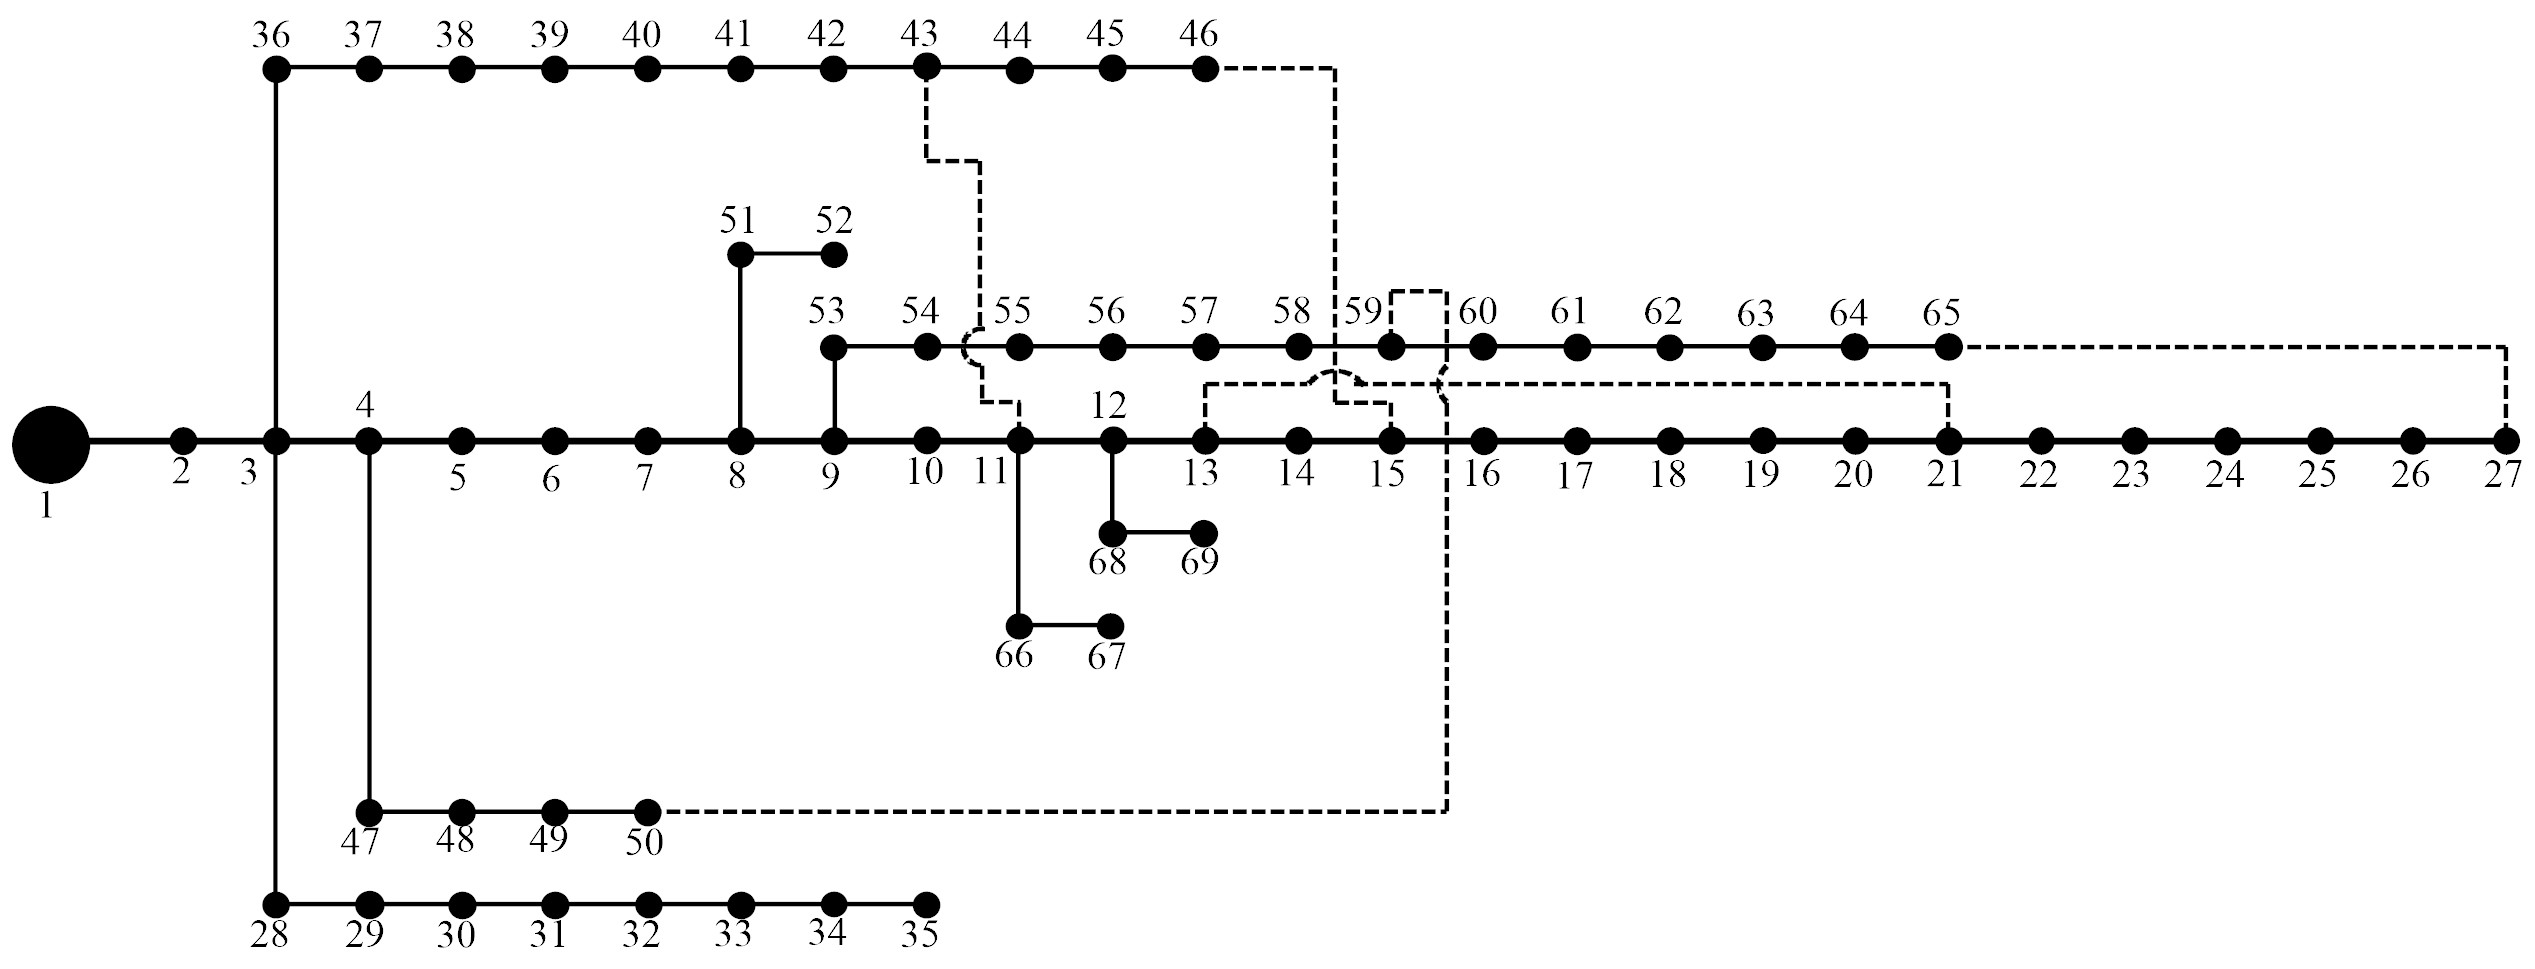
\includegraphics[width=1\textwidth]{./Figures/69bus_singleline_diagram_tieline_t1}
	\caption{Single line diagram of IEEE-69 Bus System}
	\label{fig:single69}
\end{figure}
\pagebreak
\begin{longtable}{cccccccccc}
	\caption {IEEE 69 Bus System Bus Data}
	\label{table:busdata69}
	\hline
	\multirow{3}{*}{\begin{tabular}[c]{@{}c@{}}Bus \\ No.\end{tabular}} & \multirow{3}{*}{\begin{tabular}[c]{@{}c@{}}Bus \\ Code\end{tabular}} & \multirow{3}{*}{\begin{tabular}[c]{@{}c@{}}Load\\ Type\end{tabular}} & \multicolumn{2}{c}{Load} & \multicolumn{4}{c}{Generator} & \multirow{2}{*}{\begin{tabular}[c]{@{}c@{}}Injected \\ MVAr\end{tabular}} \\  
	\cmidrule{4-5} 
	\cmidrule(lr{1em}){6-9}		 
	&  &  & \multicolumn{1}{l}{\multirow{2}{*}{MW}} & \multicolumn{1}{l}{\multirow{2}{*}{MVAr}} & \multicolumn{1}{l}{\multirow{2}{*}{MW}} & \multicolumn{1}{l}{\multirow{2}{*}{MVAr}} & \multicolumn{1}{l}{\multirow{2}{*}{Qmin}} & \multicolumn{1}{l}{\multirow{2}{*}{Qmax}} &  \\ 
	&  &  & \multicolumn{1}{l}{} & \multicolumn{1}{l}{} & \multicolumn{1}{l}{} & \multicolumn{1}{l}{} & \multicolumn{1}{l}{} & \multicolumn{1}{l}{} &  \\
	\cmidrule(lr){1-10}
	1 & 1 & - & 0 & 0 & 0 & 0 & 0 & 0 & 0 \\
	2 & 0 & Curtailable & 0 & 0 & 0 & 0 & 0 & 0 & 0 \\
	3 & 0 & Curtailable & 0 & 0 & 0 & 0 & 0 & 0 & 0 \\
	4 & 0 & Curtailable & 0 & 0 & 0 & 0 & 0 & 0 & 0 \\
	5 & 0 & Curtailable & 0 & 0 & 0 & 0 & 0 & 0 & 0 \\
	6 & 0 & Fixed & 0.0026 & 0.0022 & 0 & 0 & 0 & 0 & 0 \\
	7 & 0 & Controllable & 0.0404 & 0.0030 & 0 & 0 & 0 & 0 & 0 \\
	8 & 0 & Fixed & 0.0750 & 0.0054 & 0 & 0 & 0 & 0 & 0 \\
	9 & 0 & Fixed & 0.0300 & 0.0022 & 0 & 0 & 0 & 0 & 0 \\
	10 & 0 & Fixed & 0.0280 & 0.0019 & 0 & 0 & 0 & 0 & 0 \\
	11 & 0 & Fixed & 0.1450 & 0.1040& 0 & 0 & 0 & 0 & 0 \\
	12 & 0 & Fixed & 0.1450 & 0.1040 & 0 & 0 & 0 & 0 & 0 \\
	13 & 0 & Controllable & 0.0080 & 0.0055 & 0 & 0 & 0 & 0 & 0 \\
	14 & 0 & Controllable & 0.0080 & 0.0055 & 0 & 0 & 0 & 0 & 0 \\
	15 & 0 & Controllable & 0 & 0 & 0 & 0 & 0 & 0 & 0 \\
	16 & 0 & Controllable & 0.0455 & 0.0030 & 0 & 0 & 0 & 0 & 0 \\
	17 & 0 & Controllable & 0.0600 & 0.0350 & 0 & 0 & 0 & 0 & 0 \\
	18 & 0 & Controllable & 0.0600 & 0.0350 & 0 & 0 & 0 & 0 & 0 \\
	19 & 0 & Controllable & 0 & 0 & 0 & 0 & 0 & 0 & 0 \\
	20 & 0 & Controllable & 0.0010 & 0.0006 & 0 & 0 & 0 & 0 & 0 \\
	21 & 0 & Controllable & 0.1140 & 0.0810 & 0 & 0 & 0 & 0 & 0 \\
	22 & 0 & Controllable & 0.0530 & 0.0035 & 0 & 0 & 0 & 0 & 0 \\
	23 & 0 & Controllable & 0 & 0 & 0 & 0 & 0 & 0 & 0 \\
	24 & 0 & Controllable & 0.0280 & 0.020 & 0 & 0 & 0 & 0 & 0 \\
	25 & 0 & Controllable & 0 & 0 & 0 & 0 & 0 & 0 & 0 \\
	26 & 0 & Controllable & 0.0140 & 0.0100 & 0 & 0 & 0 & 0 & 0 \\
	27 & 0 & Curtailable & 0.0140 & 0.0100 & 0 & 0 & 0 & 0 & 0 \\
	28 & 0 & Curtailable & 0.0260 & 0.0186 & 0 & 0 & 0 & 0 & 0 \\
	29 & 0 & Curtailable & 0.0260 & 0.0186 & 0 & 0 & 0 & 0 & 0 \\
	30 & 0 & Curtailable & 0 & 0 & 0 & 0 & 0 & 0 & 0 \\
	31 & 0 & Curtailable & 0 & 0 & 0 & 0 & 0 & 0 & 0 \\
	32 & 0 & Curtailable & 0 & 0 & 0 & 0 & 0 & 0 & 0 \\
	33 & 0 & Curtailable & 0.0140 & 0.0100 & 0 & 0 & 0 & 0 & 0 \\
	\bottomrule  \\ 
	\toprule 
	34 & 0 & Curtailable & 0.0195 & 0.0140 & 0 & 0 & 0 & 0 & 0 \\
	35 & 0 & Controllable & 0.0060 & 0.0040 & 0 & 0 & 0 & 0 & 0 \\
	36 & 0 & Controllable & 0.0260 & 0.01855 & 0 & 0 & 0 & 0 & 0 \\
	37 & 0 & Controllable & 0.026 & 0.01855 & 0 & 0 & 0 & 0 & 0 \\
	38 & 0 & Controllable & 0 & 0 & 0 & 0 & 0 & 0 & 0 \\
	39 & 0 & Controllable & 0.0240 & 0.0170 & 0 & 0 & 0 & 0 & 0 \\
	40 & 0 & Controllable & 0.0240 & 0.0170 & 0 & 0 & 0 & 0 & 0 \\
	41 & 0 & Controllable & 0.0012 & 0.0100 & 0 & 0 & 0 & 0 & 0 \\
	42 & 0 & Controllable & 0 & 0 & 0 & 0 & 0 & 0 & 0 \\
%		\toprule  \\ 
%		\toprule 
	43 & 0 & Controllable & 0.0060 & 0.0043 & 0 & 0 & 0 & 0 & 0 \\
	44 & 0 & Controllable & 0 & 0 & 0 & 0 & 0 & 0 & 0 \\
	45 & 0 & Controllable & 0.03922 & 0.05263 & 0 & 0 & 0 & 0 & 0 \\
	46 & 0 & Controllable & 0.03922 & 0.0263 & 0 & 0 & 0 & 0 & 0 \\
	47 & 0 & Controllable & 0 & 0 & 0 & 0 & 0 & 0 & 0 \\
	48 & 0 & Controllable & 0.0790 & 0.0564 & 0 & 0 & 0 & 0 & 0 \\
	49 & 0 & Curtailable & 0.3847 & 0.2745 & 0 & 0 & 0 & 0 & 0 \\
	50 & 0 & Controllable & 0.3847 & 0.2745 & 0 & 0 & 0 & 0 & 0 \\
	51 & 0 & Curtailable & 0.0405 & 0.0283 & 0 & 0 & 0 & 0 & 0 \\
	52 & 0 & Curtailable & 0.0036 & 0.0027 & 0 & 0 & 0 & 0 & 0 \\
	53 & 0 & Curtailable & 0.00435 & 0.0035 & 0 & 0 & 0 & 0 & 0 \\
	54 & 0 & Curtailable & 0.0264 & 0.0190 & 0 & 0 & 0 & 0 & 0 \\
	55 & 0 & Curtailable & 0.0240 & 0.0172 & 0 & 0 & 0 & 0 & 0 \\
	56 & 0 & Curtailable & 0 & 0 & 0 & 0 & 0 & 0 & 0 \\
	57 & 0 & Fixed & 0 & 0 & 0 & 0 & 0 & 0 & 0 \\
	58 & 0 & Fixed & 0 & 0 & 0 & 0 & 0 & 0 & 0 \\
	59 & 0 & Fixed & 0.1000 & 0.0720 & 0 & 0 & 0 & 0 & 0 \\
	60 & 0 & Fixed & 0 & 0 & 0 & 0 & 0 & 0 & 0 \\
	61 & 0 & Controllable & 1.2440 & 0.8880 & 0 & 0 & 0 & 0 & 0 \\
	62 & 0 & Fixed & 0.0320 & 0.0230 & 0 & 0 & 0 & 0 & 0 \\
	63 & 0 & Fixed & 0 & 0 & 0 & 0 & 0 & 0 & 0 \\
	64 & 0 & Fixed & 0.2270 & 0.1620 & 0 & 0 & 0 & 0 & 0 \\
	65 & 0 & Fixed & 0.0590 & 0.0420 & 0 & 0 & 0 & 0 & 0 \\
	66 & 0 & Fixed & 0.0180 & 0.0130 & 0 & 0 & 0 & 0 & 0 \\
	67 & 0 & Fixed & 0.0180 & 0.0130 & 0 & 0 & 0 & 0 & 0 \\
	68 & 0 & Fixed & 0.0280 & 0.0200 & 0 & 0 & 0 & 0 & 0 \\
	69 & 0 & Controllable & 0.02800 & 0.0200 & 0 & 0 & 0 & 0 & 0 \\
	\bottomrule %[1.5pt]		
\end{longtable}
\flushleft
\item  Bus Code
\newline 1 - Slack Bus \newline 0 - Load Bus

\begin{longtable}{ccccccccc}
	\caption {IEEE 69 Bus System Line Data}
	\label{table:linedata69}
	\hline
	\multirow{4}{*}{\begin{tabular}[c]{@{}c@{}}  Line \\ No.\end{tabular}} & \multirow{4}{*}{\begin{tabular}[c]{@{}c@{}}From\\ Bus\end{tabular}} & \multirow{4}{*}{\begin{tabular}[c]{@{}c@{}}To\\ Bus\end{tabular}} & \multirow{4}{*}{\begin{tabular}[c]{@{}c@{}}R \\ (p.u)\end{tabular}} & \multirow{4}{*}{\begin{tabular}[c]{@{}c@{}}X\\ (p.u)\end{tabular}} & \multirow{4}{*}{\begin{tabular}[c]{@{}c@{}}B\\ (p.u)\end{tabular}} & \multirow{4}{*}{\begin{tabular}[c]{@{}c@{}}line code = 1\\ for lines\\ \textgreater{} 1 or \textless 1 for tr.tap\end{tabular}} & \multirow{4}{*}{\begin{tabular}[c]{@{}c@{}}Failure\\ Rate\\ (f/yr)\end{tabular}} & \multirow{4}{*}{\begin{tabular}[c]{@{}c@{}}Repair\\ Time\\ (h)\end{tabular}} \\
	
	&  &  &  &  &  &  &  &  \\
	&  &  &  &  &  &  &  &  \\
	&  &  &  &  &  &  &  &  \\
	\cmidrule{1-9} 
	1 & 1 & 2 & 0.0005 & 0.0012 & 0 & 1 & 0.0003 & 0.5 \\
	2 & 2 & 3 & 0.0005 & 0.0012 & 0 & 1 & 0.0003 & 0.5 \\
	3 & 3 & 4 & 0.0015 & 0.0036 & 0 & 1 & 0.0009 & 0.5 \\
	4 & 4 & 5 & 0.0251 & 0.0294 & 0 & 1 & 0.0156 & 0.5 \\
	5 & 5 & 6 & 0.3660 & 0.1864 & 0 & 1 & 0.2269 & 0.5 \\
	6 & 6 & 7 & 0.3811 & 0.1941 & 0 & 1 & 0.2363 & 0.5 \\
%			\toprule  \\ 
%	\toprule 
	7 & 7 & 8 & 0.0922 & 0.0470 & 0 & 1 & 0.0572 & 0.5 \\

	8 & 8 & 9 & 0.0493 & 0.0251 & 0 & 1 & 0.0306 & 0.5 \\
	
	9 & 9 & 10 & 0.8190 & 0.2707 & 0 & 1 & 0.5078 & 0.5 \\
	10 & 10 & 11 & 0.1872 & 0.0619 & 0 & 1 & 0.1161 & 0.5 \\
	11 & 11 & 12 & 0.7114 & 0.2351 & 0 & 1 & 0.4411 & 0.5 \\
	12 & 12 & 13 & 1.0300 & 0.3400 & 0 & 1 & 0.6386 & 0.5 \\
	13 & 13 & 14 & 1.0440 & 0.3450 & 0 & 1 & 0.6473 & 0.5 \\
	14 & 14 & 15 & 1.0580 & 0.3496 & 0 & 1 & 0.6560 & 0.5 \\
	15 & 15 & 16 & 0.1966 & 0.0650 & 0 & 1 & 0.1219 & 0.5 \\
	16 & 16 & 17 & 0.3744 & 0.1238 & 0 & 1 & 0.2321 & 0.5 \\
	17 & 17 & 18 & 0.0047 & 0.0016 & 0 & 1 & 0.0029 & 0.5 \\
	18 & 18 & 19 & 0.3276 & 0.1083 & 0 & 1 & 0.2031 & 0.5 \\
	19 & 19 & 20 & 0.2106 & 0.0690 & 0 & 1 & 0.1306 & 0.5 \\
	20 & 20 & 21 & 0.3416 & 0.1129 & 0 & 1 & 0.2118 & 0.5 \\
	21 & 21 & 22 & 0.0140 & 0.0046 & 0 & 1 & 0.0087 & 0.5 \\
	22 & 22 & 23 & 0.1591 & 0.0526 & 0 & 1 & 0.0986 & 0.5 \\
	23 & 23 & 24 & 0.3463 & 0.1145 & 0 & 1 & 0.2147 & 0.5 \\
	24 & 24 & 25 & 0.7488 & 0.2745 & 0 & 1 & 0.4643 & 0.5 \\
	25 & 25 & 26 & 0.3089 & 0.1021 & 0 & 1 & 0.1915 & 0.5 \\
	26 & 26 & 27 & 0.1732 & 0.0572 & 0 & 1 & 0.1074 & 0.5 \\
	27 & 3 & 28 & 0.0044 & 0.0108 & 0 & 1 & 0.0027 & 1.0 \\
		\toprule \\
	\hline
	28 & 28 & 29 & 0.0640 & 0.1565 & 0 & 1 & 0.0397 & 1.0 \\
	29 & 29 & 30 & 0.3978 & 0.1315 & 0 & 1 & 0.2466 & 1.0 \\
	30 & 30 & 31 & 0.0702 & 0.0232 & 0 & 1 & 0.0435 & 1.0 \\
	31 & 31 & 32 & 0.3510 & 0.1160 & 0 & 1 & 0.2176 & 1.0 \\
	32 & 32 & 33 & 0.8390 & 0.2816 & 0 & 1 & 0.5202 & 1.0 \\
	33 & 33 & 34 & 1.7080 & 0.5646 & 0 & 1 & 1.0590 & 1.0 \\
	34 & 34 & 35 & 1.4740 & 0.4873 & 0 & 1 & 0.9139 & 1.0 \\
	35 & 3 & 36 & 0.0044 & 0.0108 & 0 & 1 & 0.0270 & 1.0 \\
	36 & 36 & 37 & 0.0640 & 0.1565 & 0 & 1 & 0.0397 & 1.0 \\
	37 & 37 & 38 & 0.1053 & 0.1230 & 0 & 1 & 0.0653 & 1.0 \\
	38 & 38 & 39 & 0.0304 & 0.0355 & 0 & 1 & 0.0188 & 1.0\\
	39 & 39 & 40 & 0.0018 & 0.0021 & 0 & 1 & 0.0011 & 1.0 \\
	40 & 40 & 41 & 0.7283 & 0.8509 & 0 & 1 & 0.4515 & 1.0 \\
	41 & 41 & 42 & 0.3100 & 0.3623 & 0 & 1 & 0.1922 & 1.0 \\
	42 & 42 & 43 & 0.0410 & 0.0478 & 0 & 1 & 0.0254 & 1.0 \\ 
	43 & 43 & 44 & 0.0092 & 0.0116 & 0 & 1 & 0.0057 & 1.0 \\
	44 & 44 & 45 & 0.1089 & 0.1373 & 0 & 1 & 0.0675 & 1.0 \\
	45 & 45 & 46 & 0.0009 & 0.0012 & 0 & 1 & 0.0006 & 1.0 \\
	46 & 4 & 47 & 0.0034 & 0.0084 & 0 & 1 & 0.0021 & 1.0 \\
	47 & 47 & 48 & 0.0851 & 0.2083 & 0 & 1 & 0.0528 & 1.0 \\
	48 & 48 & 49 & 0.2898 & 0.7091 & 0 & 1 & 0.1797 & 1.0 \\
	49 & 49 & 50 & 0.0822 & 0.2011 & 0 & 1 & 0.5100 & 1.0 \\
	50 & 8 & 51 & 0.0928 & 0.0473 & 0 & 1 & 0.0575 & 1.0 \\
	51 & 51 & 52 & 0.3319 & 0.1114 & 0 & 1 & 0.2058 & 1.0 \\
	52 & 9 & 53 & 0.1740 & 0.0886 & 0 & 1 & 0.1079 & 1.0 \\
%			\toprule\\
%	\hline
	53 & 53 & 54 & 0.2030 & 0.1034 & 0 & 1 & 0.1259 & 1.0 \\

	54 & 54 & 55 & 0.2842 & 0.1447 & 0 & 1 & 0.1762 & 1.0 \\
	55 & 55 & 56 & 0.2813 & 0.1433 & 0 & 1 & 0.1744 & 1.0 \\
	56 & 56 & 57 & 1.5900 & 0.5337 & 0 & 1 & 0.9858 & 1.0 \\
	57 & 57 & 58 & 0.7837 & 0.263 & 0 & 1 & 0.4859 & 1.0 \\
	58 & 58 & 59 & 0.3042 & 0.1006 & 0 & 1 & 0.1886 & 1.0 \\
	59 & 59 & 60 & 0.3861 & 0.1172 & 0 & 1 & 0.2394 & 1.0 \\
	60 & 60 & 61 & 0.5075 & 0.2585 & 0 & 1 & 0.3146 & 1.0 \\
	61 & 61 & 62 & 0.0974 & 0.0496 & 0 & 1 & 0.6040 & 1.0 \\
	62 & 62 & 63 & 0.1450 & 0.0738 & 0 & 1 & 0.0899 & 1.0 \\
	63 & 63 & 64 & 0.7105 & 0.3619 & 0 & 1 & 0.4405 & 1.0 \\
	64 & 64 & 65 & 1.0410 & 0.5302 & 0 & 1 & 0.6454 & 1.0 \\
		\toprule\\
	\hline
	65 & 11 & 66 & 0.2012 & 0.0611 & 0 & 1 & 0.1247 & 1.0 \\
	66 & 66 & 67 & 0.0047 & 0.0014 & 0 & 1 & 0.0029 & 1.0 \\
	67 & 12 & 68 & 0.7394 & 0.2444 & 0 & 1 & 0.4584 & 1.0 \\
	68 & 68 & 69 & 0.0047 & 0.0016 & 0 & 1 & 0.0029 & 1.0 \\
	69* & 11 & 43 & 0.5000 & 0.5000 & 0 & 1 & 0.3100 & 1.0 \\
	70* & 13 & 21 & 0.5000 & 0.5000 & 0 & 1 & 0.3100 & 1.0 \\
	71* & 15 & 46 & 1.0000 & 1.0000 & 0 & 1 & 0.6200 & 1.0 \\
	72* & 50 & 59 & 2.0000 & 2.0000 & 0 & 1 & 1.2100 & 1.0 \\
	73* & 27 & 65 & 1.0000& 1.0000 & 0 & 1 & 0.6200 & 1.0 \\
	\bottomrule
\end{longtable}
\newline *- Tie Line	
	

%\end{document}
\appendix
%%%%%%%%%%%%%%%%%%%%%%%%%%%%%%%%%%%%%%%%%%%%%%%%%%%%%%%%%%%%

%%%%%%%%%%%%%%%%%%%%%%%%%%%%%%%%%%%%%%%%%%%%%%%%%%%%%%%%%%%%


%\plagarism
\end{document}
